\part{Основы высшей алгебры}
\chapter{Комплексные числа}
\section{Понятие комплексного числа. Арифметические операции.}
$\bullet$ \textit{\textbf{Комплексным числом} называется выражение вида $z = a+bi$, где $a, b \in \mathbb{R}$ (действительные
	числа), а $i$ --- символ, называемый \textbf{мнимой единицей}. При этом число $a$ называется \textbf{действительной частью} $z$ (Обозначение: $a = Re(z)$), а число $b$ --- \textbf{мнимой частью} $z$ (Обозначение: $b = Im(z)$).}\\\\
Множество комплексных чисел обозначается символом $\mathbb{C}$.\\\\
Если $b=0, a\ne 0$, то число $a + 0\cdot i$ считается \textbf{совпадающим с действительными числом} $a$, то есть $a + 0\cdot i = a$.\\\\
Если $b\ne 0, a\ne 0$, то число называется \textbf{мнимым}. Если при $a = 0$, то число $0+bi$ называется \textbf{чисто мнимым} и обозначается через $bi$, то есть ($0+bi = bi$).\\\\
Пусть $z_1 = a_1 + b_1 i$, $z_2 = a_2 + b_2 i$ --- два комплексных числа. Комплексные числа $z_1$ и $z_2$ \textbf{равны}, если равны их действительные и мнимые части, то есть $z_1 = z_2 \Longleftrightarrow a_1 = a_2,\ b_1 = b_2$.\\\\
$\bullet$ \textit{\textbf{Суммой комлексных чисел} $z_1$ и $z_2$ называется число: $$z_1 + z_2 = (a_1 + a_2) + (b_1 + b_2) i.$$}
\textbf{\textit{Свойства сложения комплексных чисел:}}\begin{enumerate}
	\item $z_1 + z_2 = z_2 + z_1$. \begin{Proof}
		$z_1 + z_2 = (a_1 + a_2) + (b_1 + b_2) i = (a_2 + a_1) + (b_2 + b_1) i = z_2 + z_1$.
	\end{Proof}
	\item $(z_1 + z_2) + z_3 = z_1 + (z_2 + z_3)$.
\end{enumerate}
Операция сложения порождает операцию вычитания:\\\\
$\bullet$ \textit{\textbf{Разностью комплексных чисел} $z_1$ и $z_2$ называется число: $$z_1 - z_2 = (a_1 - a_2) + (b_1 - b_2) i.$$ }
$\bullet$ \textit{\textbf{Произведением комплексных чисел} $z_1$ и $z_2$ называется число: $$z_1 \cdot z_2 = (a_1 \cdot a_2 - b_1 \cdot b_2) + (a_1 \cdot b_2 + b_1 \cdot a_2) i.$$ }\\\\
\textbf{\textit{Свойства произведения комплексных чисел:}}\begin{enumerate}
	\item $z_1\cdot z_2 = z_2\cdot z_1$.
	\item $(z_1\cdot z_2)\cdot z_3 = z_1\cdot (z_2\cdot z_3)$.
	\item $(z_1 + z_2)\cdot z_3 = z_1\cdot z_3 + z_2 \cdot z_3$.
\end{enumerate}
Из определения произведения комплексных чисел следует, что $i^2 = (0 + 1i)(0+1i) = -1 + 0i = -1$. То есть во множестве $\mathbb{C}$ уравнение $x^2 + 1 = 0$ имеет решение $x = i$.\\\\
Если числа $z_1$ и $z_2$ действительные, то операции сложения и умножения этих чисел совпадают с операциями сложения и умножения действительных чисел.\\\\
Пусть $z = a+ bi$ --- комплексное число.\\\\
$\bullet$ \textit{Комплексное число $\overline{z} = a - bi$ называется \textbf{сопряжённым для комплексного числа $z$}.}\\\\
Из определения следует, что $\overline{z} = z$. Следовательно, можно говорить о паре сопряжённых друг другу комплексных чисел.\\\\
Операция умножения комплексных чисел порождает операцию деления:\\\\
$\bullet$ \textit{\textbf{Частным от деления комплексных чисел} $z_1$ и $z_2$ называется число $z_3$ такое, что $z_2 \cdot z_3 = z_1$. }\\\\
Тогда \begin{multline*}
	\dfrac{z_1}{z_2} = \dfrac{a_1 + b_1 i}{a_2 + b_2 i} = \text{[домножим на сопряженное]} = \dfrac{(a_1 + b_1 i)(a_2 - b_2 i)}{(a_2 + b_2 i)(a_2 - b_2 i)}=\\= \dfrac{a_1\cdot a_2 + b_1 \cdot b_2}{a_2^2 + b_2 ^ 2} + \dfrac{b_1 \cdot a_2 - a_1 \cdot b_2}{a_2^2 + b_2^2}i.
\end{multline*}
\textbf{\textit{Свойства сопряжённых комплексных чисел:}}\begin{enumerate}
	\item $z + \overline{z} = 2\cdot Re(z)$.\\
	$z - \overline{z} = 2\cdot Im(z)\cdot i$.\begin{Proof}
		Если $z = a + bi$, то $z + \overline{z} = (a+bi) + (a-bi) = (a+a) + (b-b)i = 2a$.
	\end{Proof}
	\item $z = \overline{z}\Longleftrightarrow z\in \mathbb{R}$.\begin{Proof}
		$\Rightarrow)$ Пусть $z = \overline{z}$, тогда $z + \overline{z} = 0 = 2\cdot Im(z)\cdot i\Rightarrow Im(z) = 0\Rightarrow z\in\mathbb{R}$.\\
		$\Leftarrow)$ Пусть $z\in\mathbb{R}$. Следовательно, $z = a + 0i\Rightarrow \overline{z} = a - 0i = a = z$.
	\end{Proof}
	\item $\overline{z_1} + \overline{z_2} = \overline{z_1 + z_2};\ \overline{z_1} - \overline{z_2} = \overline{z_1 - z_2}$.\begin{Proof}
		Пусть $z_1 = (a_1 + b_1i),\ z_2 = a_2 + b_2 i \Rightarrow z_1 + z_2 = (a_1 + a_2) + (b_1 + b_2) i$. Тогда $\overline{z_1} + \overline{z_2} = (a_1 - b_1i) + (a_2 - b_2 i) = (a_1 + a_2) - (b_1 +b_2) i = \overline{z_1 + z_2}$.
	\end{Proof}
	\item $\overline{z_1}\cdot\overline{z_2} = \overline{z_1\cdot z_2}$.\\\\
	$\dfrac{\overline{z_1}}{\overline{z_2}} = \overline{\left(\dfrac{z_1}{z_2}\right)}$.
\end{enumerate}











\section{Комплексная плоскость. Тригонометрическая и экспоненциальная
	форма записи комплексного числа.}
Пусть на плоскости задана ДПСК $Oxy$. Каждому комплексному числу вида $z = a + bi$ поставим в соответствие координаты $(a,b)$. С другой стороны, каждой точке с координатами $(a, b)$ мы можем поставить в соответствие комплексное число $z = a + bi$.\\\\
$\bullet$ \textit{Плоскость, точки которой рассматриваются как комплексные числа, называется \textbf{комплексной плоскостью}. При этом ось $Ox$ называется \textbf{действительной осью}, а ось $Oy$ --- \textbf{мнимой осью}, так как на ней располагаются чисто мнимые числа.}
\begin{center}
	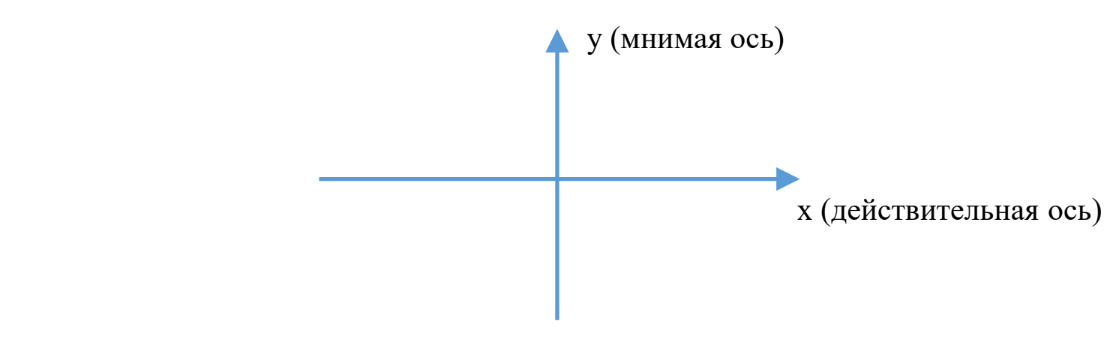
\includegraphics[scale=0.3]{images/kdpsk.png}
\end{center}
Построим на комплексной плоскости соответствующую полярную систему координат. И пусть $z = a + bi$ --- некоторое комплексное число. Тогда этому числу на комплексной плоскости соответствует точка, имеющая декартовы координаты $(a, b)$ и полярные координаты $(\rho, \varphi)$. \\Следовательно, $\begin{cases}
	a = \rho\cdot cos \varphi,\\
	b = \rho\cdot sin \varphi;
\end{cases}$, где $\rho = \sqrt{a^2 + b^2}$, а угол $\varphi$ можно найти, решив систему: $\begin{cases}
	cos \varphi = \dfrac{a}{\sqrt{a^2 + b^2}},\\\\
	sin \varphi = \dfrac{b}{\sqrt{a^2 + b^2}};
\end{cases}$\\\\
Тогда комплексное число $z$ представимо в виде: $z = a+bi= \rho\cdot cos \varphi + i\cdot \rho\cdot sin\varphi = \rho(cos\varphi + i\cdot sin\varphi)$.\\\\
$\bullet$ \textit{Форма вида $z = \rho(cos\varphi + i\cdot sin\varphi)$ называется \textbf{тригонометрической формой записи комплексного числа}. В свою очередь, форма вида $z = a + bi$ называется \textbf{алгебраической формой записи комплексного числа.} }\\\\
$\bullet$ \textit{Полярный радиус $\rho$ называется \textbf{модулем комплексного числа}. А полярный угол $\varphi$ называтся \textbf{аргументом комплексного числа} (Обозначения: $|z|$ и $Arg(z)$ соответственно).}\\\\
Аргумент комплексного числа определён с точностью до слагаемого $2\pi k$. Значение аргумента, принадлежащее полуотрезку $(\pi;\pi]$, называют \textbf{главным} значением аргумента.\\\\
\textbf{\textit{Свойства значения аргумента:}}\begin{enumerate}
	\item $|z| = |\overline{z}|, Arg(z) = -Arg(\overline{z})$.\begin{Proof}
		Доказательство следует оз определения числа $z$.
	\end{Proof}
	\item $|z|^2 = z\cdot\overline{z}$.\begin{Proof}
		Пусть $z = a + bi$, тогда $\overline{z} = a - bi$.\\
		$z\cdot\overline{z} = (a+bi)(a-bi) = a^2 - (bi)^2 = a^2 + b^2 = |z|^2$.
	\end{Proof}
	\item \textit{Модуль разности комплексных чисел равен расстоянию между точками на комплексной плоскости, соответствующих этим числам, то есть $$|z_1 - z_2| = \sqrt{(a_1 - a_2)^2 + (b_1 - b_2)^2}.$$}
	\begin{Proof}
		Пусть $\begin{cases}
			z_1 = a_1 + b_1 i,\\
			z_2 = a_2 + b_2 i;
		\end{cases}\Rightarrow z_1 - z_2 = (a_1 - a_2) + (b_1 - b_2)i\Rightarrow |z_1 - z_2| = \sqrt{(a_1 - a_2)^2 + (b_1 - b_2)^2} = \rho(z_1, z_2)$.
	\end{Proof}
	\item $|z_1\cdot z_2| = |z_1|\cdot|z_2|$.\\
	$Arg(z_1\cdot z_2) = Arg(z_1) + Arg(z_2).$\begin{Proof}
		Запишем числа $z_1$ и $z_2$ в тригонометрической форме: $z_1 = \rho_1(cos\varphi_1 + i\cdot sin\varphi_1),\ z_2 = \rho_2(cos\varphi_2 + i\cdot sin\varphi_2)$. Отсюда получаем, что $|z_1| = \rho_1,\ |z_2| = \rho_2,\ Arg(z_1) = \varphi_1,\ Arg(z_2) = \varphi_2$. \\Тогда произведение чисел $z_1$ и $z_2$ в тригонометрической форме имеет вид: $z_1\cdot z_2 = \rho_1\rho_2((cos\varphi_1cos\varphi_2 - sin\varphi_1sin\varphi_2) + i(cos\varphi_1sin\varphi_2 + sin\varphi_1cos\varphi_2)) = \rho_1\rho_2(cos(\varphi_1 + \varphi_2) + i\cdot sin(\varphi_1 + \varphi_2))$. \\Из полученного следует, что $|z_1\cdot z_2| = \rho_1\rho_2 = |z_1|\cdot|z_2|$, а $Arg(z_1\cdot z_2) = \varphi_1 + \varphi_2 = Arg(z_1) + Arg(z_2)$.
	\end{Proof}
	\item $\left | \dfrac{z_1}{z_2} \right | = \dfrac{|z_1|}{|z_2|}, Arg(\dfrac{z_1}{z_2}) = Arg(z_1) - Arg(z_2)$.\begin{Proof}
		Доказательство проводится по аналогии с предыдущим пунктом.
	\end{Proof}
	\newtheorem*{cor6_3_1}{Следствие}\begin{cor6_3_1} $z^{-1} = \dfrac{1}{z} = \dfrac{1(cos\varphi + i\cdot sin\varphi)}{\rho(cos\varphi + i\cdot sin\varphi)} = \dfrac{1}{\rho}(cos(-\varphi) + i\cdot sin(\varphi))$.
	\end{cor6_3_1}
	\item \textbf{Формула Маувра}\\
	\textit{Если $z = \rho(cos\varphi + i\cdot sin\varphi)$, то $\forall\ n \in \mathbb{Z}\ z^n = \rho^n(cos(n\varphi) + i\cdot sin(n\varphi))$}.\begin{Proof}
		Доказательство следует по индукции из пункта 4 и следствия.
	\end{Proof}
\end{enumerate}
$\bullet$ $e^{i\varphi}=cos\varphi + i\cdot sin\varphi$ --- \textit{\textbf{формула Эйлера}}.\\
$\bullet$ $z = \rho e^{i\varphi}$ ---\textit{ \textbf{экспоненциальная форма записи комплексного числа}}.





\section{Извлечение корня из комплексного числа.}
Пусть $z$ --- некоторое комплексное число.\\\\
$\bullet$ \textit{\textbf{Корнем n-ой степени из комплексного числа} $z$ называется число $z_0$ такое, что $z_0$ в степени $n$ равно Самому комплексному числу $z$. То есть $z_0^n = z$.}
\newtheorem*{t6_3_1}{Теорема}\begin{t6_3_1} Извлечение корня $n$-ой степени из комплексного числа $z = \rho(cos\varphi + i\cdot sin\varphi)$ всегда возможно и, при $z\ne 0$, даёт
	ровно $n$ различных значений: $$z_k = \sqrt[n]{\rho}\left(cos\left (\dfrac{\varphi + 2\pi k}{n}\right ) + i\cdot sin\left(\dfrac{\varphi + 2\pi k}{n}\right) \right),\ k=0,1,\dots,n-1,$$
	где $\sqrt[n]{\rho}$ --- действительное положительное число, $n$-ая степень которого равна $\rho$.
\end{t6_3_1}\begin{Proof}
	Пусть существует корень $n$-ой степени из числа $z$ и он равен $z_0 = \rho_0(cos\varphi_0 + i\cdot sin\varphi_0)$. Тогда по формуле Маувра $z_0^n = \rho_0^n(cos(n\varphi_0) + i\cdot sin(n\varphi_0)) = \rho(cos(\varphi) + i\cdot sin(\varphi))$.\\\\
	Если комплексные числа равны, то их модули равны, а аргументы могут отличаться на $2\pi k$, где $k \in \mathbb{Z}$. Следовательно, $\rho_0^n = \rho,\ n\varphi_0 = \varphi + 2\pi k \Rightarrow \varphi_0 = \dfrac{\varphi + 2 \pi k}{n}, k\in \mathbb{Z}\Rightarrow z_k$ является корнем $n$-ой степени числа $z$.\\\\
	Покажем, что при $k\in [0, n-1]$ числа $z_k$ различные:\\\\
	Пусть существуют 2 числа $p$ и $q$ из отрезка $[0, n-1]$ такие, что $z_p = z_q$, и пусть $0\leqslant p < q < n\Rightarrow \exists l \in \mathbb{N} : \dfrac{\varphi + 2\pi q}{n} = \dfrac{\varphi + 2\pi p}{n} + 2\pi l\Rightarrow 2 \pi l = \dfrac{2\pi ( q - p)}{n}$. А так как $q < n$ и $p < n$, то $\dfrac{q-p}{n} < 1$. Следовательно, $l < 1$, что является противоречием с тем, что $l \in \mathbb{N}$.\\\\
	Покажем, что при $k \not\in [0, n-1]$ новых значений $z_k$ мы не получим:\\\\
	Разделим $k$ на $n$ с остатком. Пусть $p$ и $q$ --- частное и остаток при делении соответственно. Тогда $z = p \cdot n + q, 0 \leqslant q < n$.\\
	Тогда $Arg(z_k) = \varphi_k = \dfrac{\varphi + 2\pi k}{n} = \dfrac{\varphi + 2\pi (p n + q)}{n} = \dfrac{\varphi + 2\pi q}{n} + 2\pi p \Rightarrow z_k = z_q^n\Rightarrow$ новых корней мы не получим.
\end{Proof}















\chapter{Алгебраические структуры}

\section{Бинарные отношения.}
Пусть $X$, $Y$ --- два непустых множества.\\\\
$\bullet$ \textit{\textbf{Декартовым произведением} множества $X$ на множество $Y$ называется мно- } \\ \textit{жество всех упорядоченных пар $(x,y)$, где $x$ $\in$ $X$ и $y$ $\in$ $Y$. Обозначается $X$ $\times$ $Y$. То есть}
\begin{center}
	$X\times Y$ = \{$(x,y)$ | $x$ $\in$ $X$, $y$ $\in$ $Y$\}.   
\end{center}
$\bullet$ \textit{Декартово произведение множества $X$ на себя называется \textbf{декартовым квадратом} множества $X$. То есть}
\begin{center}
	$X^2$ = $X$ $\times$ $X$.
\end{center}
$\bullet$ \textit{\textbf{Бинарным отношением,} заданным на множестве $X$, называется подмножество декартового квадрата множества $X$. Обозначается символом $\sigma$ (сигма)}.\\\\
Если $\sigma$ --- бинарное отношение на множестве $X$ ($\sigma$ $\subseteq$ $X^2$) и пара $(x,y)$ $\in$ $\sigma$, то говорят, что элемент $x$ находится в отношении $\sigma$ с элементом $y$. Записывается $x$ $\sigma$ $y$.\\\\
$\bullet$ \textit{Бинарное отношение $\sigma$, заданное на множестве $X$, называется:}
\begin{enumerate}
	\item \textit{\textbf{рефлексивным}, если $\forall x$ $\in$ $X$ : $x\sigma x$}
	\item \textit{\textbf{транзитивным}, если из соотношений $x \sigma y$, $y \sigma z$ $\Rightarrow$ $x$$\sigma$$z$}
	\item \textit{\textbf{симметричным}, если из $x$$\sigma$$y$ $\Rightarrow$ $y$$\sigma$$x$}
	\item \textit{\textbf{антисимметричным}, если из $x$$\sigma$$y$, $y$$\sigma$$x$ $\Rightarrow$ $x$ = $y$}
\end{enumerate}
$\bullet$ \textit{\textbf{Бинарным отношением эквивалентности} называется рефлексивное, транзитивное, симметричное бинарное отношение. Обозначается $\sim$.}\\\\
Пусть на множестве $X$ задано бинарное отношение эквивалентности и пусть $x$ --- некоторый элемент множества $X$.\\\\
$\bullet$ \textit{Подмножество множества $X$, состоящее из всех элементов, эквивалентных элементу $x$, называется \textbf{классом эквивалентности}, содержащим этот $x$. Обозначается $\overline{x}$. То есть}
\begin{center}
	$\overline{x}$ = \{$x'$ $\in$ $X$ | $x'$ $\sim$ $x$\}.
\end{center}
$\bullet$ \textit{Любой элемент множества $\overline{x}$ называется \textbf{представителем} класса $\overline{x}$}. \\\\
$\bullet$ \textit{Если множество $X$ представимо в виде объединения попарно непересекающихся подмножеств, то говорят, что множество $X$ \textbf{разбивается} на эти подмножества.}
\newtheorem*{t6_1}{Теорема}\begin{t6_1} Пусть $X$ --- некоторое множество, на котором задано отношение эквивалентности, тогда оно разбивается на классы эквивалентности по этому бинарному отношению. \end{t6_1} \begin{Proof} 
	Множество $X$ всегда можно представить в виде $X$ = $\underset{x \in X}{\bigcup}\underbrace{\{x\}}_{\subset \
		\overline{x}}$ $\subseteq$ $\underset{x \in X}{\bigcup}\overline{x}$ $\subset$ $X$ $\Rightarrow$ $X$ = $\underset{x \in X}{\bigcup}\overline{x}$ \\\
	Покажем, что два 2 класса эквивалентности $\overline{x_1}$ и $\overline{x_2}$ или совпадают, или не переекаются.\\\\
	Пусть $\overline{x_1}$ $\cap$ $\overline{x_2}$ $\not=$ $\varnothing$ $\Rightarrow$ $\exists$ $x$ $\in$ $\overline{x_1}$ $\cap$ $\overline{x_2}$ $\Rightarrow$ $x$ $\in$ $\overline{x_1}$, $x$ $\in$ $\overline{x_2}$ $\Rightarrow$ $x$ $\sim$ $x_1$, $x$ $\sim$ $x_2$ $\overset{\textit{симм.}}{\Rightarrow}$ $x_1$ $\sim$ $x$, $x$ $\sim$ $x_2$ $\overset{\textit{транз.}}{\Rightarrow}$ $x_1$ $\sim$ $x_2$ $\Rightarrow$ $\forall x$ $\in$ $\overline{x_1}$, $x$ $\sim$ $x_1$, $x_1$ $\sim$ $x_2$ $\overset{\textit{транз.}}{\Rightarrow}$  $x$ $\sim$ $x_2$ $\Rightarrow$ $x$ $\in$ $\overline{x_2}$ $\Rightarrow$ $\overline{x_1}$ $\subseteq$ $\overline{x_2}$.\\\\
	С другой стороны, так как бинарное отношение эквивалентности симметрично, то из этого следует, что $x_1$ $\sim$ $x_2$ $\Rightarrow$ $x_2$ $\sim$ $x_1$ $\Rightarrow$ $\overline{x_2}$ $\subseteq$ $\overline{x_1}$ $\Rightarrow$ $\overline{x_1}$ = $\overline{x_2}$.
\end{Proof}\\\\
$\bullet$ \textit{Бинарное отношение, заданное на множестве $X$, называется \textbf{отношением порядка}, если оно рефлексивно, транзитивно и антисимметрично. Обозначается $\le$.}\\\\
Если $\forall x,y$ $\in$ $X$ или $x$ $\le$ $y$, или $y$ $\le$ $x$, то множество $X$ называется \textbf{линейно упорядоченным}. Но пара $(x,y)$ может и не находиться в бинарном отношении порядка. Если такая пара существует, то $X$ --- \textbf{частично упорядоченное множество.}\\\\
Пусть на множестве $X$ задано бинарное отношение порядка.\\\\
$\bullet$ \textit{\textbf{Наибольшим элементом} множества $X$ называется такой элемент $n$ $\in$ $X$, что \\ $\forall x$ $\in$ $X$ : $x\le n$.}\\\\
$\bullet$ \textit{\textbf{Максимальным элементом} множества $X$ называется такой элемент $m$ $\in$ $X$, что $\nexists$ $x\in X$,  $x\not=$ $m$ : $m$ $\le$ $x$.}\\\\
\textbf{Замечание:} Максимальных элементов во множестве может быть несколько, а наибольший элемент, если он существует, только один.





\section{Отображения.}
Пусть $X$, $Y$ --- некоторые непустые множества.\\\\
$\bullet$ \textit{Говорят, что определено однозначное \textbf{отображение} множества $X$ на множество $Y$, если каждому элементу из множества $X$ постав\'{и}м в соответствие только один элемент из множества $Y$. Обозначение: $f$: $X$ $\rightarrow$ $Y$}.\\\\
Заметим, что $f$ $\subset$ $X$ $\times$ $Y$. А также $\forall x$ $\in$ $X$ $\exists!y$ $\in$ $Y$ : $(x,y)$ $\in$ $f$.\\\\
$\bullet$ \textit{Если отображение f элемент x ставит в соответствие элементу y, то говорят, что $y$ --- \textbf{образ} элемента x, а $x$ --- \textbf{прообраз} элемента y. \\Обозначение образа: $\{f(x)\ |\ \forall x\in X \} = ImX = f(x)$.\\
	Обозначение прообраза: $f(x)$ = $y$ или $f$: $x$ $\mapsto$ $y$.}\\\\
Из определения отображения следует, что $f(x)$ $\subseteq$ $Y$.\\\\
$\bullet$ \textit{Отображение $f: X\rightarrow Y$ называется \textbf{инъективным}, если $\forall x_1, x_2$ $\in$ $X$, $x_1$ $\not=$ $x_2$ $\Rightarrow$ \\ $f(x_1)$ $\not=$ $f(x_2)$}.\\\\
$\bullet$ \textit{Отображение $f: X\rightarrow Y$ называется \textbf{сюръективным}, если $\forall$$y$ $\in$ $Y$  $\exists$$x$ $\in$ $X$ : $f(x) = y$}.\\\\
$\bullet$ \textit{Отображение $f: X\rightarrow Y$ называется \textbf{биективным}, если оно инъективно и сюръективно} \textit{(взаимнооднозначное соответствие)}.\\\\
$\bullet$ \textit{Два отображения $f$: $X$ $\rightarrow$ $Y$ и $g$: $X'$ $\rightarrow$ $Y'$ называются \textbf{равными}, если $X$ = $X'$}, \\ \textit{$Y$ = $Y'$ и $\forall x$ $\in$ $X$ $f(x)$ = $g(x)$.}\\\\
Пусть $f$: $X$ $\rightarrow$ $Y$ --- некоторое отображение. $X'$ $\subseteq$ $X$. Тогда \\\\
$\bullet$ \textit{Отображение $g$: $X' \rightarrow Y'$ называется \textbf{ограничением отображения} $f$ на множестве $X'$, если $\forall x$ $\in$ $X'$ : $g(x) = f(x)$. Обозначение: $f|_\textit{X'}$. Само же отображение $f:X\rightarrow Y$ называется \textbf{продолжением отображения} $g$ на множестве $X$.}\\\\
Пусть $f$: $X$ $\rightarrow$ $Y$ и $g$: $Y$ $\rightarrow$ $Z$. Тогда\\\\
$\bullet$ \textit{Отображение $g$ $\circ$ $f$ : $X$ $\rightarrow$ $Z$ которое работает так, что $\forall x$ $\in$ $X$ $(g \circ f)(x)$ = $g(f(x))$, называется \textbf{композицией отображений} $g$ и $f$.}\\\\
Из определения следует, что композиция $g$ и $f$ отображена.
\newtheorem*{t6_2}{Теорема}\begin{t6_2} Пусть $f$: $X$ $\rightarrow$ $Y$, $g$: $Y$ $\rightarrow$ $Z$ и $h = g \circ f$. Тогда
	\begin{enumerate}
		\item если $f$ и $g$ инъективны, то $h$ инъективно;
		\item если $f$ и $g$ сюръективны, то $h$ сюръективно;
		\item если $f$ и $g$ биективны, то $h$ биективно.
	\end{enumerate}
\end{t6_2} \begin{Proof} \begin{enumerate}
		\item Пусть $f$ и $g$ --- инъекции, тогда $$\forall x_1, x_2 \in X\ x_1 \not= x_2 \Rightarrow f(x_1) \not= f(x_2),\ g(f(x_1)) \not= g(f(x_2))$$ Следовательно, $h$ инъективно, так как $$(g\circ f)(x_1) = g(f(x_1)) = h(x_1),\quad (g\circ f)(x_2) = g(f(x_2)) = h(x_2),$$ и $h(x_1) \not= h(x_2)$.
		\item Пусть $f$ и $g$ --- сюръекции и пусть $z_0$ --- произвольный элемент множества $Z$. Так как $g$ --- сюръекция, то для $z_0$ $\exists y_0$ $\in$ $Y$ такой, что $g(y_0) = z_0$. А так как $f$ --- сюръекция, то для этого элемента $y_0$ $\exists x_0$ $\in$ $X$ такой, что $f(x_0) = y_0$ Тогда $$\forall z_0 \in Z\ \exists x_0 : h(x_0) = (g \circ f)(x_0) = g(f(x_0)) = g(y_0) = z_0.$$ Следовательно, $h$ --- сюръекция.
		\item Биективность вытекает из двух предыдущих пунктов.
\end{enumerate} \end{Proof}\\
$\bullet$ \textit{Отображение $e_X : X$ $\rightarrow$ $X$ такое, что $\forall x$ $\in$ $X$ $e_X(x) = x$ называется \textbf{тождественным отображением} множества $X$}.\\\\
Пусть $f$ : $X$ $\rightarrow$ $Y$ --- некоторое отображение. \\\\
$\bullet$ \textit{Отображение $g$ : $Y$ $\rightarrow$ $X$ называется \textbf{обратным} для отображения $f$, если $g \circ f$ = $e_X$, $f \circ g$ = $e_Y$.}
\newtheorem*{t6_2_2}{Теорема}\begin{t6_2_2} Отображение $f$ : $X$ $\rightarrow$ $Y$ имеет обратное $\Longleftrightarrow$ оно биективно.
\end{t6_2_2} \begin{Proof} $\Rightarrow$) Пусть отображение $f$: $X$ $\rightarrow$ $Y$ имеет обратное отображение $g$ : $Y$ $\rightarrow$ $X$. Покажем, что $f$ инъективно и сюръективно. \begin{enumerate}
		\item Инъективность.\\ 
		Возьмем произвольные $x_1, x_2$ $\in$ $X$ такие, что $x_1 \not= x_2$. Покажем, что $f(x_1) \not= f(x_2)$.\\
		От противного. Предположим, что $f(x_1) = f(x_2)$.
		Возьмем элемент $x_1$, тогда $$x_1 = e_X(x_1) = (g \circ f)(x_1) = g(f(x_1)) = g(f(x_2)) = (g \circ f)(x_2) = e_X(x_2) = x_2,$$ что противоречит выбранным $x_1$ и $x_2$. Следовательно, $f(x_1) \not= f(x_2)$ и $f$ --- инъекция.
		\item Сюръективность.\\ 
		$$\forall y_0 \in Y\ y_0 = e_Y (y_0) = (f \circ g)(y_0) = f(g(y_0)).$$ Тогда $\exists x_0$ $\in$ $X$ : $x_0$= $g(y_0)$, $f(x_0) = y_0$ и $f$ --- сюръекция
	\end{enumerate}
	Из этих двух пунктов получаем, что $f$ --- биекция.\\\\
	$\Leftarrow$) Пусть отображение $f$: $X$ $\rightarrow$ $Y$ биективное. Тогда $\forall$$y_0$ $\in$ $Y$ $\exists$$!$ $x_0$ $\in$ $X$  [существование следует из сюръекции, а единственность из инъекции]: $f(x_0) = y_0$. Следовательно, существует отображение $g$: $Y$ $\rightarrow$ $X$ такое, что $g(y_0) = x_0$, то есть обратное для $f$. \\\\
	Тогда $$\forall y_0 \in Y \ (f \circ g)(y_0) = f(g(y_0)) = f(x_0) = y_0 = e_Y(y_0) \Rightarrow e_Y = f \circ g.$$
	$$\forall x_0 \in X\ (g \circ f)(x_0) =  g(f(x_0))  =  g(y_0)  =  x_0  =  e_X(x_0) \Rightarrow e_X = g \circ f.$$
\end{Proof}
\newtheorem*{t6_2_3}{Теорема}\begin{t6_2_3} Пусть $f$: $X$ $\rightarrow$ $Y$, $g$: $Y$ $\rightarrow$ $Z$, $h$: $Z$ $\rightarrow$ $U$, тогда $h \circ (g \circ f)$ = $(h \circ g) \circ f$.
\end{t6_2_3} \begin{Proof} 
	Так как $g \circ f$ : $X$ $\rightarrow$ $Z$, тогда $h \circ (g \circ f)$ : $X$ $\rightarrow$ $U$, а из
	$h \circ g$ : $Y$ $\rightarrow$ $U$ следует, что\\ $h \circ (g \circ f)$ : $X$ $\rightarrow$ $U$.
	Следовательно, множества совпадают. Значит справедливы равенства
	$\forall x \in X$ $$(h \circ (g \circ f))(x) = h((g \circ f)(x)) = h(g(f(x))),$$
	$$((h \circ g) \circ f)(x) = (h \circ g)(f(x)) = h(g(f(x))).$$
\end{Proof}





\section{Бинарная алгебраическая операция.}
Пусть $X$ --- некоторое непустое множество.\\\\
$\bullet$ \textit{Отображение $f$ : $X^2$ $\rightarrow$ $X$, ставящее каждой упорядоченной паре $(a,b) \in X^2$ в соответствие элемент $c\in X$ называется \textbf{бинарной алгебраической операцией.} \\ Обозначается $f$ : $(a,b)$ $\mapsto$ $c$ или $f(a,b) = c$}.\\\\
Для произвольной алгебраической операции $a * b = c$, где $*$ --- символ символ (они могут выглядеть по-разному: $+, -, *$ и так далее).\\\\
$\bullet$ \textit{Алгебраическая операция $*$ называется} \begin{enumerate}
	\item \textit{\textbf{ассоциативной,} если $(a*b)*c = a*(b*c)$ $\quad\forall a, b, c \in X$;}
	\item \textit{\textbf{коммутативной,} если $a*b = b*a$ $\quad\forall a, b \in X$.}
\end{enumerate}
$\bullet$ \textit{Элемент $n$ $\in$ $X$ называется \textbf{нейтральным} элементом в $X$ относительно операции $*$, если $n * x = x * n = x\quad\forall x$ $\in$ $X$.}
\newtheorem*{t6_3}{Теорема}\begin{t6_3} В множестве $X$ относительно алгебраической операции $*$ может существовать не более одного нейтрального элемента. \end{t6_3} 
\begin{Proof} От противного. Пусть в $X$ относительно операции $*$ существуют два нейтральных элемента $n_1$ и $n_2$. Тогда $n_1 * n_2 = n_1$, а $n_2 * n_1 = n_2$ $\Rightarrow$ $n_1 = n_2$, так как алгебраическая операция --- однозначное отображение. \end{Proof} \\\\
Пусть во множестве $X$ определена операция $*$, относительно которой в $X$ существует нейтральный элемент.\\\\
$\bullet$ \textit{Элемент $a'\in X$ называется \textbf{симметричным} для элемента $a\in X$ относительно операции $*$, если $a' * a$ = $a * a'$ = $n$.}
\newtheorem*{t6_3_2}{Теорема}\begin{t6_3_2} Если на множестве $X$ алгебраическая операция $*$ ассоциативна и существует нейтралный элемент, то для любого элемента $a\in X$ может существовать не более одного симметричного элемента.  \end{t6_3_2} 
\begin{Proof}
	От противного. Пусть $b_1, b_2$ --- два элемента, симметричных элементу $a$ относительно операции $*$. Тогда $b_1 * a$ = $a * b_1$ = $n$, $b_2 * a$ = $a * b_2$ = $n$ $\Rightarrow$ $b_1 = b_1 * n = b_1 * (a * b_2) = (b_1 * a) * b_2 = n * b_2 = b_2$ $\Rightarrow$ $b_1 = b_2$ $\Rightarrow$ симметричный элемент, если он есть, единственный. \end{Proof} \\\\
Рассмотрим некоторые операции и их характеристику:\begin{center}
	%\begin{table}[]
	\begin{tabular}{|c|c|c|}
		\hline
		Операция & Аддитивная запись & Мультипликативная запись  \\
		\hline
		Знак & $+$ & $\cdot$ \\
		Название & сложение & умножение \\
		Результат & сумма & произведение \\
		Нейтральный элемент & $0$ & $1$ \\
		Симметричный элемент & $-a$ (противоположный) & $a^{-1}$ (обратный) \\
		\hline
	\end{tabular}
	%\end{table}
\end{center}
$\bullet$ \textit{Множество $X$ c определенной на нем алгебраической операцией $*$ является \textbf{алгебраической структурой}. Обозначается $(X, *)$}.\\\\
\textbf{Замечание}: Современная алгебра занимается изучением алгебраических структур.



\section{Группа.}
$\bullet$ \textit{Непустое множество $G$ с заданной на нем алгебраической операцией $*$ называется \textbf{группой}}, если \begin{enumerate}
	\item \textit{операция $*$ ассоциативна};
	\item \textit{в $G$ $\exists$ нейтральный элемент относительно операции $*$};
	\item \textit{в $G$ $\forall$$a$ $\exists$ симметричный ему элемент $a'$ относительно операции $*$}.
\end{enumerate}
\textit{Обозначение: $(G, *)$}.\\\\
$\bullet$ \textit{Если при этом операция $*$ является коммутативной, то группа называется \textbf{абелевой.}} \\\\
$\bullet$ \textit{Если группа содержит конечное количество элементов, то группа называется \textbf{конечной.}} \\\\
$\bullet$ \textit{Количество элементов в конечной группе называется \textbf{порядком} группы}.\\\\
\textbf{\textit{Свойства групп:}}\begin{enumerate}
	\item \textit{В группе существует единственный нейтральный элемент и для любого элемента группы в ней существует единственный симметричный}
	\begin{Proof} Доказательство следует из теорем о единственности нейтрального и
		симметричного элементов. \end{Proof}
	\item \textit{Пусть $a, b$ --- произвольные элементы группы $(G, *)$. $a'$--- элемент, симметричный элементу $a$ относительно $*$. Тогда уравнения}
	$$a * x = b \hspace{2 cm} x*a = b$$
	\textit{имеют единственные решения соответственно $$x_0 = a' * b\hspace{2cm} x_0 = b * a'.$$}
	\begin{Proof} Доказательство проведем для первого уравнения, для второго доказательство аналогично.
		Покажем, что $x_0 = a' * b$ --- решение уравнения $a * x = b$. Для проверки подставим: $a * x_0 = a * (a' * b) = (a * a') * b = n * b = b$. Cледовательно, $a' * b$ --- решение. \\
		Покажем, что это решение единственное. \\
		От противного. Предположим, что уравнение $a * x = b$ имеет еще одно некоторое решение $x_1$. Тогда 
		$a * x_1 = b$ $\Rightarrow$ $x_0 = a' * b = a' * (a * x_1) = (a' * a) * x_1 = n * x_1 = x_1$, $x_0 = x_1$ $\Rightarrow$ решение единственное.
	\end{Proof}
	\item \textbf{Закон сокращения в группе:}\begin{itemize}
		\item если $a * b = a * c$, то $b = c$;
		\item если $b * a = c * a$, то $b = c$.
	\end{itemize}
	\begin{Proof} Пусть $a'$ --- элемент, симметричный элементу $a$ относительно операции $*$. Тогда, $b = n * b = (a' * a) * b = a' * (a * b) = [ a*b = a*c ] = a' * (a * c) = (a' * a) * c = n * c = c.$ \end{Proof}
\end{enumerate}
Пусть $(G, *)$ --- некоторая группа.\\\\
$\bullet$ \textit{Непустое подмножество множества $G$ называется \textbf{подгруппой} группы $G$, если она сама является группой относительно той же операции $*$}.
\newtheorem*{t7_4_1}{Лемма}\begin{t7_4_1} Пусть $(H, *)$ --- подгруппа группы $(G, *).$ Тогда нейтральный элемент $n_G$ совпадает с нейтральным элементом $n_H$. \end{t7_4_1} 
\begin{Proof} Так как $n_H$ --- нейтральный элемент в группе $H$, то $n_H * n_H = n_H$. Так как $n_H$ $\in$ $H\subseteq G$, то в $G$ существует единственный симметричный ему элемент $n'_H$. То есть $n_H * n'_H = n_G$. Тогда $n_G = n_H * n'_H = (n_H * n_H) * n'_H = n_H * (n_H * n'_H) = n_H * n_G = n_H.$ \end{Proof}
\newtheorem*{t7_4_2}{Теорема}\begin{t7_4_2} Пусть $(G, *)$ --- группа. Непустое подмножество $H$ множества $G$ является подгруппой группы $G$ $\Longleftrightarrow$ выполняются следующие условия: \begin{enumerate}
		\item операция $*$ определена в $H$, то есть $\forall$$a, b$ $\in$ $H\quad a * b$ $\in$ $H$. 
		\item $\forall$$a$ $\in$ $H$ симметричный ему в $G$ элемент $a'_G$ $\in$ $H$.
\end{enumerate} \end{t7_4_2} 
\begin{Proof} $\Rightarrow$) \begin{enumerate}
		\item Пусть $(H, *)$ --- подгруппа группы $(G, *)$ $\Rightarrow$ $(H,*)$ сама является группой относительно операции * $\Rightarrow$ операция $*$ в $H$ определена.
		\item Покажем, что $\forall$$a$ $\in$ $H$, $a'_G$ $\in$ $H$.\\ Так как $a$ $\in$ $H$ и $(H,*)$ --- группа, то в $H$ существует единственный симметричный для $a$ элемент $a'_H$, то есть $a * a'_H = a'_H * a = n_H = $ [ по лемме ] $ = n_G$ $\Rightarrow$ элемент $a'_H$ является симметричным для элемента $a$ в группе $G$, но по первому свойству группы элемент имеет только единственный сииметричный ему элемент. Следовательно, $a'_G = a'_H$, причем $a'_H$ $\in$ $H$.
	\end{enumerate}
	$\Leftarrow$) Пусть $H$ --- непустое подмножество множества $G$. $(H, *)$ --- группа. \begin{enumerate}
		\item Операция $*$ в $H$ определена по первому условию достаточности;
		\item Операция $*$ в $H$ ассоциативна, так как она ассоциативна в $G$;
		\item Нейтральный элемент группы $G$ $(n_G)$ является нейтральным и во множестве $H$, так как $\forall$$a$ $\in$ $H$ $\exists$$a'$: $a * a' = n_G$ $\in$ $H$;
		\item Элемент $a'_G$ $\in$ $H$ и является симметричным для $a$ в $H$.
	\end{enumerate}
	Следовательно, $(H,*)$ --- группа, а так как $H\subseteq G$, то $(H,*)$ --- подгруппа группы $(G,*)$.
\end{Proof}
\section{Кольцо.}
$\bullet$ \textit{Непустое множество $K$ с определенными на нем операциями сложения и умножения называется \textbf{кольцом}, если} \begin{enumerate}
	\item $(K, +)$ --- \textit{абелева группа};
	\item \textit{операция умножения дистрибутивна относительно операции сложения, то есть} $\forall a,b,c \in K\\
	a\cdot (b+c) = a\cdot b + a\cdot c;\\
	(b+c)\cdot a = b\cdot a + c\cdot a.$
\end{enumerate}
$\bullet$ \textit{Абелева группа $(K,+)$ называется \textbf{аддитивной группой} кольца $K$.}\\\\
$\bullet$ \textit{Если умножение коммутативно в $K$, то кольцо называется \textbf{коммутативным}. Если умножение ассоциативно --- \textbf{ассоциативным}.}\\\\
\textit{\textbf{Свойства колец:}}\begin{enumerate}
	\item $a\cdot 0 = 0\cdot a = 0\quad \forall a \in K$.
	\begin{Proof}
		$a\cdot 0 + a\cdot 0 = a\cdot (0+0) = a\cdot 0 = a\cdot 0 + 0 \Rightarrow a\cdot 0 = 0$ по закону сокращения в группе $(K, +)$.
	\end{Proof}\\
	Обратное утверждение для данного свойства, вообще говоря, неверно.
\end{enumerate}
$\bullet$ \textit{Если существуют числа $a,b\in K$ такие, что $a\cdot b = 0$, при этом $a\ne 0$, $b\ne 0$, то эти числа называются \textbf{делителями нуля}.}
\begin{enumerate}
	\item[2.] $a\cdot (-b) = (-a)\cdot b = -(a\cdot b)$.
	\begin{Proof}
		$(-a)\cdot b + a\cdot b = b((-a) + a) = 0\cdot b = 0$. Следовательно, элемент $(-a)\cdot b$ является симметричным относительно сложения для элемента $a\cdot b$.
	\end{Proof}
	\item[3.] \textit{Умножение дистрибутивно относительно вычитания, то есть} $a-b = a + (-b)$.\begin{Proof}
		$(a-b)\cdot c = (a + (-b))\cdot c = a\cdot c + (-b)\cdot c = a\cdot c + (-b\cdot c) = a\cdot c - b\cdot c$.
	\end{Proof}
	\item[4.] \textit{Кольцо может иметь не более одной единицы. Если кольцо состоит из более, чем одного элемента, то этот элемент не является нулем.}
	\begin{Proof}
		Если в кольце существует нейтральный элемент, то он
		единственный. Следовательно, если единица --- нейтральный элемент для операции умножения, то эта единица единственная.\\\\
		Пусть кольцо $K$ состоит из более, чем одного элемента, и имеет единицу равную нулю $(1 = 0)$, тогда $\forall a \in K$ $a\cdot 1 = a\cdot 0 = 0$. Следовательно, $K = \{a\}$, то есть в кольце $K$ будет существовать только 1 элемент, что является противоречием.
	\end{Proof}
\end{enumerate}
Пусть $K$ --- кольцо с единицей.\\\\
$\bullet$ \textit{Если для $a\in K$ существует $a^{-1}\in K$, то $a$ называется \textbf{обратимым элементом} кольца $K$, а элемент $a^{-1}$ --- \textbf{обратным элементом} для $a$.}
\newtheorem*{7_5_1}{Теорема}\begin{7_5_1}
	В ассоциативном кольце с единицей множество $K^*$
	всех обратимых элементов кольца $K$
	является группой относительно операции умножения $(K^*, \cdot)$. 
\end{7_5_1}\begin{Proof}
	Докажем все аксиомы определения.\begin{enumerate}
		\item Так как $1\cdot 1 = 1$, то элемент 1 обратимый. Следовательно, множество $K^*$ непустое.
		\item Пусть $a,b\in K^*$. Тогда $\exists a^{-1}, b^{-1} \in K$ и $b^{-1}a^{-1}\in K$ (так как в кольце определена операция умножения).\\
		$(b^{-1}a^{-1})(ab) = b^{-1}(a^{-1}a)b = [a^{-1}a = n = 1] = b^{-1}\cdot 1\cdot b = b^{-1}b = 1$. Аналогично $(ab)(b^{-1}a^{-1}) = 1$. Следовательно, элемент $b^{-1}a^{-1}$ обратный для $ab$ и $ab\in K^*$.
		\item Умножение в $K^*$ ассоциативно, так как оно ассоциативно в $K$.
		\item 1 --- нейтральный относительно умножения элемент.
		\item $\forall a \in K^* \exists a^{-1}\in K : aa^{-1} = 1$. Следовательно, элемент $a$ обратимый для $a^{-1}$, $a \in K^*$. Тогда в $K^*$ $\forall a\quad \exists a^{-1} : aa^{-1} = 1$.
	\end{enumerate}
\end{Proof}\\
$\bullet$ \textit{Группа обратимых элементов ассоциативного кольца с единицей $(K^*, \cdot )$ называется
	\textbf{мультипликативной группой} кольца $K$.}\\\\
$\bullet$\textit{ Подмножество $L$ кольца $K$ называется \textbf{подкольцом} кольца $K$, если $(L, +, \cdot )$ само
	является кольцом относительно тех же операций, что и $K$.}
\newtheorem*{7_5_2}{Теорема}\begin{7_5_2}
	Непустое подмножество $L\subseteq K$, если $K$ --- кольцо, является подкольцом $\Longleftrightarrow$ выполняются следующие условия:\begin{enumerate}
		\item операции $+$ и $\cdot$ определены в L, то есть $\forall a,b\quad \in L\ a+b \in L, a\cdot b \in L$;
		\item $\forall a \in L\quad (-a) \in L$.
	\end{enumerate}
\end{7_5_2}
\begin{Proof}
	$\Rightarrow)$  Пусть $(L, +, \cdot)$ --- подкольцо кольца $(K, +, \cdot)$. Тогда $(L, +, \cdot)$ само является кольцом. Следовательно\begin{enumerate}
		\item операции определены;
		\item $\forall a \in L\quad (-a) \in L$, так как $(L, +)$ --- абелева группа.
	\end{enumerate}
	$\Leftarrow)$ Из пунктов 1 и 2 достаточности следует, что $(L, +)$ --- подгруппа группы $(K, +)$, и она является абелевой группой.
	Дистрибутивность относительно умножения в $L$ следует из дистрибутивности в $K$, так как $L\subseteq K$. Следовательно, так как все аксиомы кольца
	выполняются в $(L, +, \cdot)$, то оно является кольцом, а так как $L\subseteq K$, то $(L, +, \cdot)$ является подкольцом кольца $(K, +, \cdot)$. 
\end{Proof}
\section{Поле.}
$\bullet$ \textit{Множество $P$, содержащее не менее двух элементов, с заданными на нем операциями сложения и умножения называется \textbf{полем}, если}\begin{enumerate}
	\item $(P, +)$ --- \textit{абелева группа};
	\item $(P\backslash \{0\}, \cdot)$ --- \textit{абелева группа};
	\item \textit{умножение дистрибутивно относительно сложения, то есть} $\forall a,b,c \in P\\
	(a+b)\cdot c = a\cdot c + b\cdot c$. 
\end{enumerate}
То есть поле --- обязательно кольцо ассоциативное, коммутативное, с единицей, каждый ненулевой элемент которого обратим.\\\\
\textit{\textbf{Свойства полей:}}\begin{enumerate}
	\item \textit{В поле нет делителей нуля}.\begin{Proof}
		Пусть для некоторых $a,b\in P$ выполняется $a\cdot b = 0$. Предположим, что $a\ne 0$. Следовательно, $\exists a^{-1} \in P : 0 = a^{-1}\cdot 0 = a^{-1}\cdot (a\cdot b) = (a^{-1}\cdot a)\cdot b = 1\cdot b = b$, то есть $b = 0$.
	\end{Proof}
	\item \textbf{Закон сокращения:} \textit{Если $a\ne 0$ и $a\cdot b = a\cdot c$, то $b=c\quad \forall b,c \in P$.}
	\item \textit{Если $a\ne 0$, то уравнение $a\cdot x = b$ имеет единственное решение $a^{-1}\cdot b\quad \forall b \in P$.}
	\begin{Proof}
		Если $b\ne 0$ и $c \ne 0$, то утверждения 2 и 3 справедливы по свойствам группы $(P\backslash \{0\}, \cdot)$.\\
		Если $b = 0$ и $c = 0$, то утверждения 2 и 3 справедливы, так как в поле нет делителей нуля.
	\end{Proof}
\end{enumerate}
$\bullet$ \textit{Непустое подмножество $F$ поля $(P, +,\cdot)$ называется \textbf{подполем} поля $P$, если $F$ является полем относительно тех же операций, что и поле $P$. В свою очередь, поле $P$ называется \textbf{расширением} поля $F$.}
\newtheorem*{7_6_1}{Теорема}\begin{7_6_1}
	Непустое подмножество $F$ поля $P$, содержащее не менее двух элементов, является подполем поля $P$, если \begin{enumerate}
		\item в $F$ определенв операции сложения и умножения, то есть $\forall a,b \in F\quad (a + b),~(a\cdot~b)~\in~F$;
		\item $\forall a \in F\quad (-a) \in F$;
		\item $\forall a \in F, a\ne 0 \quad a^{-1} \in F$. 
	\end{enumerate}
\end{7_6_1} \begin{Proof}
	Доказательство следует из критерия подгрупп. Аналогично схожей теореме для подкольца.
\end{Proof}\\\\
$\bullet$ \textit{Число $n\in \mathbb{N}$, которое обозначает минимальное количество единиц в поле $P$, дающих в
	сумме нуль (то есть $\underbrace{1 + 1 + \ldots + 1}_{n} = 0$), называется \textbf{характеристикой} поля.}\\\\ Если такого числа не существует,
характеристику поля считают равной нулю.\\\\
\textbf{\textit{Свойства характеристики поля:}}\begin{enumerate}
	\item \textit{Все конечные поля имеют положительную характеристику. Бесконечные поля могут иметь как
		нулевую, так и положительную характеристику.}
	\begin{Proof}
		Пусть поле положительное и конечное. Тогда $\exists k, m : \underbrace{1 + 1 + \ldots + 1}_{k} = \underbrace{1 + 1 + \ldots + 1}_{m}$. Пусть $m > k$, тогда $0 = \underbrace{1 + 1 + \ldots + 1}_{m-k}$. Следовательно, $\exists n : \underbrace{1 + 1 + \ldots + 1}_{n} = 0$, то есть характеристика поля положительная.
	\end{Proof}
	\item \textit{Если число $n\in \mathbb{N}$ является характеристикой поля $P$, то число $n$ простое.}\begin{Proof}
		Пусть $n = pk$, где $p,k \in \mathbb{R}$. Тогда $\underbrace{1+1+\ldots+1}_{n} = 0$, то есть $\underbrace{(1+1+\ldots+1)}_{p}\cdot\\ \cdot \underbrace{(1+1+\ldots+1)}_{k} = 0$. Следовательно, из первого свойства или первый множитель равен нулю, или второй множитель равен нулю, что является противоречием с тем, что число $n$ минимальное. Значит число $n$ простое.
	\end{Proof}
\end{enumerate}


\chapter{Кольцо многочленов}
\section{Определение и простейшие свойства многочленов.}
Пусть $P$ --- некоторое поле.\\\\ 
$\bullet$ \textit{\textbf{Многочленом над полем $P$} называется выражение вида $$a_nx^n + a_{n-1}x^{n-1}
	+...+ a_1x + a_0,$$ где $a_i$ --- элементы поля $P$, а $x$ --- символ. При этом элементы $a_i$ называются
	\textbf{коэффициентами многочлена}, символ $x$ – \textbf{переменной многочлена}, а отдельные
	выражения $a_ix^i$
	– \textbf{членами многочлена}. Обозначение многочлена: $f(x)$}\\\\
Множество всех многочленов над полем $P$ с переменной $x$ обозначается как $P[x]$.\\\\
$\bullet$ \textit{Число $k$ называется \textbf{степенью многочлена}, если $a_k \not= 0$, а коэффициенты при более
	высоких степенях $x$ равны нулю, если они есть. Обозначение: $deg(f(x))$. Коэффициент $a_k$ при этом называется \textbf{старшим коэффициентом многочлена $f(x)$}, а коэффициент $a_0$ --- \textbf{свободным членом} 
	многочлена $f(x)$}.\\\\
$\bullet$ \textit{Если все коэффициенты равны нулю, то многочлен называется \textbf{нулевым.}}\\\\ Степень нулевого 
многочлена не определена. Любой элемент поля $P$ можно рассматривать как многочлен нулевой 
степени.\\\\
$\bullet$ \textit{Два многочлена называются\textbf{ равными}, если равны их степени и коэффициенты при 
	одинаковых степенях переменной.}\\\\
Рассмотрим два многочлена из $P[x]$: $f(x) = a_nx^n
+ \ldots + a_1x + a_0$ и $g(x) = b_kx^k
+ \ldots + b_1x + b_0$. Пусть $a_n\ne0$ и $b_k \, \not= 0$, то есть $deg (f(x)) = n, deg(g(x)) k$,
и пусть $n \geqslant k$ (для определённости).\\\\
$\bullet $ \textit{\textbf{Суммой многочленов} $f(x)$ и $g(x)$ называется многочлен $$(f+g)(x)= c_nx^n + … + c_1x + c_0,$$ 
	где $$c_i= \begin{cases}
		a_i+b_i, \, 0 \leqslant i \leqslant k,\\
		a_i, k+1 \leqslant i \leqslant n.\\
	\end{cases}$$}\\\\
Из определения суммы многочленов следует, что $deg(f+g)(x) \leqslant \max\{ deg(f(x)), deg(g(x))\}$.\\\\
$\bullet$ \textit{\textbf{Произведением многочленов $f(x)$ и $g(x)$} называется многочлен $$(f\cdot g)(x) = d_{n+k}x^{n+k} + \ldots + d_1x + d_0,$$ где $d_i = \sum_{i=s+l}a_sb_l$, $i = \overline{0, n+k}$.}\\\\
Из определения произведения многочленов следует, что $deg(f(x)\cdot g(x)) = deg(f(x))+deg(g(x))$.
\newtheorem*{t8_3_1}{Теорема}\begin{t8_3_1}
	Множество $P[x]$ является ассоциативным, коммутативным кольцом с единицей 
	относительно операций сложения и умножения многочленов. 
\end{t8_3_1}
\begin{Proof}
	Из определения суммы и произведения следует, что результат операций тоже является многочленом, следовательно, эти операции определены в $P[x]$.\\
	Операция $+$ коммутативна, так как $(f + g)(x) = (a_n + b_n)x^n + … + (a_1 + b_1)x + (a_0 + b_0) = (b_n + a_n)x_n + … + (b_1
	+ a_1)x + (b_0 + a_0) = (g + f)(x)$. Остальные аксиомы кольца доказываются аналогично.\\
	При этом нейтральным элементом для сложения является нулевой многочлен, а для умножения --- многочлен $f(x) = 1$.\\
	Симметричным относительно сложения для многочлена $f(x)$ является многочлен $-f(x)$ (все коэффициенты с противоположным
	знаком).
\end{Proof}\\\\
Из определения сложения и умножения многочленов и последней теоремы следует, что многочлен 
есть сумма его членов, а каждый его член – произведение $a_ix^i$. Следовательно, порядок членов в многочлене 
можно менять произвольно, члены с нулевым коэффициентом можно произвольно опускать и 
вводить в многочлен.\\\\
$\bullet$ \textit{Кольцо $(P[x], +, \cdot)$ называется \textbf{кольцом многочленов} над полем $P$ от одной переменной $x$.}\\\\
\textit{\textbf{Свойства кольца многочленов:}}
\begin{enumerate}
	\item \textit{В кольце многочленов $P[x]$ нет делителей нуля.}
	\begin{Proof}
		Из определения произведения многочленов следует, что старший коэффициент произведения ненулевых членов равен произведению ненулевых старших коэффициентов множителей, которые, в свою очередь, являются элементами поля $P$. А так как в поле делителей нуля нет, то произведение ненулевых многочленов 
		будет являться ненулевым многочленом. 
	\end{Proof}
	\item \textit{Ненулевой многочлен $f(x)$ обратим в кольце многочленов $\Longleftrightarrow deg(f(x)) = 0$.}
	\begin{Proof}
		$\Rightarrow)$ Пусть $f(x)$ обратим, то есть $\exists f^{-1}(x)\in P[x]:f(x)\cdot f^{-1}(x) = 1 \Rightarrow\\ \begin{cases}
			deg(f(x)\cdot f^{-1}(x)) = deg(1) = 0 ,\\
			deg(f(x)\cdot f^{-1}(x)) = deg(f(x)) + deg(f^{-1}(x)) = 0.
		\end{cases}$ 
		Так как степень больше нуля быть не может, то $deg(f) = 0.$\\\\
		$\Leftarrow)$ Пусть $deg(f) = 0$. Тогда $f(x) = a_0 \in  P \backslash \{0\}$, а для элемента $a \exists  a_0^{-1} \in \, P \, \Rightarrow \exists g(x) = a_0^{-1} \in P[x]$. При этом $f(x)\cdot g(x) = a\cdot a^{-1} = 1$. Значит $g(x) = f^{-1}(x)$.
	\end{Proof}\\\\
	Из второго свойства становится понятным, что сокращать многочлен можно только на константу.
	\item \textbf{Закон сокращения:} \textit{Если $h(x) \not=  0$ и $f(x)\cdot h(x) = g(x)\cdot h(x)$, то $f(x) = g(x)$.}
	\begin{Proof}
		Если $f(x)h(x) = g(x)h(x)$, то $f(x)h(x) - g(x)h(x) = 0$. Тогда $h(x)(f(x) - g(x)) = 0$, а так как по первому 
		свойству делителей нуля в кольце многочленов нет и $h(x) \not= 0$ по условию, то $f(x) - g(x) = 0$ и $f(x) = g(x)$. 
	\end{Proof}
\end{enumerate}

\section{Деление с остатком в кольце многочленов.}
Пусть $P$ --- некоторое поле.
\newtheorem*{t8_2_1}{Теорема о делении с остатком}\begin{t8_2_1}
	Для любых двух многочленов $f(x)$ и $g(x)\in P[x]$, причем $g(x)\not= 0$, существует единственная пара многочленов $q(x)$ и $r(x)$ такая, что \begin{center}
		$f(x) = g(x)\cdot q(x) + r(x)$, где $r(x) = 0$ или $deg(r(x)) < deg(g(x)).$ 
	\end{center}
\end{t8_2_1}
\begin{Proof}
	\begin{enumerate}
		\item Существование.\\\\
		Если $f(x) = 0$ или $deg(f(x)) < deg(g(x))$, то утверждение верно при $q(x) = 0$ и $r(x) = 
		f(x)$, так как $f(x) = 0\cdot g(x) + f(x)$.\\\\
		Пусть $deg(f(x)) \geqslant deg(g(x))$, $f(x) = a_nx^n + \ldots + a_1x + a_0$ и $g(x) = b_kx^k
		+ \ldots + b_1x + b_0$. При этом $a_n\ne 0$ и $b_n \ne0 \Rightarrow
		deg(f(x)) = n, deg(g(x)) = k$, и пусть $n \geqslant k$.\\\\
		Рассмотрим многочлен $\dfrac{a_n}{b_x}\cdot x^{n-k} \cdot g(x)$. Его степень равна $n$, а старший коэффициент равен $a_n$. Тогда, составив многочлен $f_1(x)=f(x)- \frac{a_n}{b_x}\cdot x^{n-k}\cdot g(x)$, получим, что $f_1(x)$ или нулевой, или $deg(f_1(x))=k_1<n = deg(f(x)).$\\\\
		Если $k_1 \geqslant k$, то обозначим старший коэффициент $f_1(x)$ за $C^{(1)}$. Построим многочлен $f_2(x) = f_1(x) - \dfrac{C^{(1)}}{b_k}\cdot x^{k_1-k}\cdot g(x).$
		Он также является либо нулевым многочленом, либо $deg(f_2(x)) = k_2 < k_1 = deg(f_1(x)).$\\\\
		Аналогично, если $k_2 \geqslant k$, построим $f_3(x)$. Так как на каждом шаге степень $f_i(x)$ понижается, но при этом у ненулевых многочленов степень неотрицательная, продолжим этот процесс до тех пор, пока на $s+1$ шаге не 
		получим многочлен $f_{s+1}(x) = f_s(x) - \dfrac{C^{(s)}}{b_k}\cdot x^{k_s-k}\cdot g(x),$ который либо нулевой, либо степени меньшей, чем $k~=~deg(g(x))$.\\\\
		Сложим полученные равенства: $f_1(x) + \ldots + f_s(x) + f_{s+1}(x) = f(x) + f_1(x) + \ldots + f_s(x) - g(x)( \dfrac{a_n}{b_k}x^{n-k} + \ldots + 
		\dfrac{C^{(s)}}{b_k}x^{k_s-k}) \Rightarrow$ [вычтем с обеих сторон $f_1(x) + \ldots + f_s(x)$]  $\Rightarrow\ f_{s+1}(x) = f(x) - g(x)( \dfrac{a_n}{b_k}x^{n-k} + \ldots + \dfrac{C^{(s)}}{b_k}x^{k_s-k})$.\\\\
		Пусть $f_{s+1}(x) = r(x), (\frac{ a_n}{b_k}x^{n-k} + … + \frac{C^{(s)}}{b_k}x^{k_{s-k}}) = q(x)$. Выразив $f(x)$, получим $f(x) = g(x)\cdot q(x) + r(x)$. При 
		этом многочлен $r(x)$ либо нулевой, либо со степенью меньшей, чем $g(x)$.
		\item Единственность.\\\\
		От противного. Пусть для $f(x)$ и $g(x)$ существует два различных разложения:
		\begin{enumerate}
			\item $f(x) = q_1(x)\cdot g(x) + r_1(x)$;
			\item $f(x) = q_2(x)\cdot g(x) + r_2(x)$,
		\end{enumerate}
		$r_1(x) \ne 0, r_2(x)\ne0$ или $deg(r_1(x)) < deg(g(x))$, $deg(r_2(x)) < deg(g(x))$.\\\\
		Вычтем из первого второе:
		$0 = (q_1(x) - q_2(x))g(x) + (r_1(x) - r_2(x)) \Rightarrow (q_2(x) - q_1(x))g(x) = r_1(x) - r_2(x)$.\\\\
		Если $q_2(x) - q_1(x) \not= 0$, то $r_1(x) - r_2(x) \not= 0$ (вспомним, что $g(x)$ по условию теоремы тоже не равно 
		нулю). Тогда так как равные многочлены имеют равные степени по определению равенства многочленов, то 
		$deg((q_2(x) - q_1(x))g(x)) = deg(q_2(x) - q_1(x)) + deg(g(x)) = deg(r_1(x) - r_2(x)) \geqslant deg(g(x))$ и $ deg(r_1(x) - r_2(x)) \leqslant max \{deg(r_1), deg(r_2)\} \leqslant
		deg(g(x))$ --- противоречие. Тогда $q_2(x) - q_1(x) = 0\Rightarrow r_1(x) - r_2(x) = 0 \Rightarrow$ разложения совпадают. 
	\end{enumerate}
\end{Proof}\\
$\bullet$ \textit{Многочлен $q(x)$ в теореме называется \textbf{частным} при делении многочлена $f(x)$ на $g(x)$, а многочлен $r(x)$ --- \textbf{остатком}}.

\section{Делимость многочленов. НОД. Алгоритм Евклида.}
$\bullet$ \textit{Говорят, что многочлен $g(x)$ \textbf{делит} многочлен $f(x)$ (или $f(x)$ \textbf{делится} на $g(x)$), если остаток при делении $f(x)$ на $g(x)$ равен нулю. Обозначения: $g(x)|f(x)$ или $f(x)\ \vdots\ g(x)$.}\\\\
\textit{\textbf{Свойства делимости многочленов:}}\\
\begin{enumerate}
	\item  $g(x)|f(x) \Longleftrightarrow \exists \varphi(x) \in P[x]: f(x) = \varphi(x)\cdot g(x).$
	\begin{Proof} 
		$\Rightarrow )$ Пусть $g(x)|f(x)$. Тогда по теореме о делении с остатком $\exists! q(x), r(x) : f(x) = g(x)\cdot q(x) + r(x)$, при этом, так как $g(x)|f(x)$, то 
		$r(x) = 0$, а многочлен $q(x)$ обозначим как $\varphi(x)$. Тогда $f(x) = \varphi(x)\cdot g(x)$.\\\\
		$\Leftarrow)$ Пусть $\exists \varphi(x) : f(x) = g(x)\cdot \varphi(x)$. Тогда $f(x) = g(x)\cdot \psi(x) + 0 =$ [ по аналогичной теореме ] $= g(x)\cdot q(x) + r(x)$,
		где $r(x) = 0$. По теореме о делении с остатком такое представление $f(x)$ единственное и $g(x)|f(x)$.
	\end{Proof}
	\item \textit{Если $h(x)|g(x)$, а $g(x)|f(x)$, то $h(x)|f(x)$. }
	\begin{Proof} 
		Если $g(x)|f(x)$, то $\exists \varphi_1(x): f(x) = g(x)\cdot\varphi_1(x);$\\
		Если $h(x)|g(x)$, то $\exists \varphi_2(x): h(x) = f(x)\cdot\varphi_2(x) = [f(x) = g(x)\cdot\varphi_1(x)] = g(x)\cdot\varphi_1(x)\cdot\varphi_2(x) = 
		g(x)\cdot(\varphi_1(x)\cdot\varphi_2(x)) = [\varphi_1(x)\cdot\varphi_2(x) = \varphi(x)] = g(x)\cdot\varphi(x)$. \\Следовательно, по свойству 1 $h(x)|f(x).$
	\end{Proof}
	\item  \textit{Если $h(x)|f(x)$, $h(x)|g(x)$, то $h(x)|(f(x) \pm g(x)).$}
	\begin{Proof} 
		Пусть $h(x)|f(x)$. Тогда $\exists \varphi_1(x): f(x) = h(x)\cdot\varphi_1(x).$ Если $h(x)|g(x)$, то $\exists \varphi_2(x): g(x) = h(x)\cdot\varphi_2(x)$. Из полученных равенств следует, что $f(x) \pm g(x) = h(x)\cdot\varphi_1(x)\pm h(x)\cdot\varphi_2(x) = h(x)\cdot(\varphi_1(x) \pm \varphi_2(x)) = [\varphi_1(x) \pm \varphi_2(x) = \varphi(x)] = h(x)\cdot\varphi(x)\Rightarrow h(x)|(f(x) \pm g(x)).$
	\end{Proof}
	\item \textit{Если $g(x)|f(x)$, то $\forall \, h(x) \in P[x]: \, g(x)|f(x)\cdot h(x)$.}
	\begin{Proof} 
		Пусть $g(x)|f(x)$. Тогда $\exists \varphi(x): f(x) = g(x)\cdot\varphi(x) \Rightarrow f(x)\cdot h(x) = g(x)\cdot (\varphi(x)\cdot h(x)) = [\varphi(x)\cdot h(x) = \varphi_1(x)] = g(x)\cdot\varphi_1(x) \Rightarrow g(x)|f(x)\cdot h(x).$ 
	\end{Proof}
	\item \textit{Если $g(x)|f(x)$, то $\forall a \in P,\ne 0\quad (a\cdot g(x))|f(x).$}
	\begin{Proof} 
		Пусть $g(x)|f(x)$. Тогда $\exists \varphi(x):  f(x) = g(x)\cdot\varphi(x) = \varphi(x)\cdot1\cdot g(x) = (\varphi(x)\cdot a^{-1})\cdot (a\cdot g(x)) = \varphi(x)\cdot (a\cdot a^{-1})\cdot g(x) = [\varphi(x)\cdot a^{-1} = \varphi_1(x)] = \varphi_1(x)\cdot(a\cdot g(x)) \Rightarrow (a\cdot g(x))|f(x).$ 
	\end{Proof}
	\item \textit{Два ненулевых многочлена $f(x)$ и $g(x)$ делят друг друга $\Longleftrightarrow \exists a \in P, \ne 0: f(x) = a\cdot g(x).$}
	\begin{Proof} 
		$\Rightarrow)$ Многочлены $g(x)$ и $f(x)$ делят друг друга, то есть $g(x)|f(x)$, тогда $\exists \, \varphi(x): f(x) = \varphi(x)\cdot g(x)$. Следовательно, $deg(f(x)) = deg(\varphi(x)) + 
		deg(g(x)) \geqslant deg(g(x)).$\\ По аналогичным рассуждениям $deg(g(x)) \geqslant deg(f(x))$.\\ 
		Так как многочлены делят друг друга, то $deg(g(x)) = deg(f(x)) \Rightarrow deg(\varphi(x)) = 0 \Rightarrow \exists a \in P, \ne 0: \varphi(x) = a \Rightarrow f(x) = a\cdot g(x).$\\
		$\Leftarrow)$ Пусть $f(x) = a\cdot g(x)$. Тогда $a = \varphi(x) \Longrightarrow f(x) = \varphi(x)\cdot g(x) \Rightarrow g(x)|f(x)$ по первому свойству.\\
		С другой стороны, так как $a \not= 0$, то $\exists a^{-1}: g(x) = a^{-1}\cdot f(x) = [a^{-1} = \varphi_1(x)] = \varphi_1(x)\cdot f(x)$. Следовательно, $f(x)|g(x).$
	\end{Proof}
\end{enumerate}
$\bullet$ \textit{Многочлен $d(x)$ называется \textbf{общим делителем} $f(x)$ и $g(x)$, если он делит каждый из 
	этих многочленов. Многочлены нулевой степени являются общими делителями для любых многочленов $f(x)$ и $g(x)$. Если других общих делителей нет, то многочлены $f(x)$ и $g(x)$ называюися \textbf{взаимно простыми}.}\\\\
$\bullet$ \textit{\textbf{Наибольшим общим делителем (НОД)} многочленов $f(x)$ и $g(x)$ называется их общий делитель, который делится на любой другой общий делитель этих многочленов.}
\newtheorem*{831}{Теорема}\begin{831}
	НОД любых двух ненулевых многочленов $f(x)$ и $g(x)$ всегда существует и определён с 
	точностью до умножения на ненулевой постоянный элемент поля $P$.
\end{831}
\begin{Proof}\begin{enumerate}
		\item Существование.\\
		Поделим $f(x)$ на $g(x)$ с остатком, и пусть $q_1(x)$ и $r_1(x)$ --- частное и остаток при этом делении соответственно, то есть $f(x) = q_1(x)\cdot g(x) + r_1(x)$. Если $r_1(x) \not= 0$, то $deg(r_1(x)) < deg(g(x))$, тогда разделим $g(x)$ на $r_1(x)$ с остатком, и пусть $q_2(x)$ и $r_2(x)$ --- частное и 
		остаток при этом делении. Если $r_2(x) \not= 0$, то $deg(r_2(x)) < deg(r_1(x))$, тогда разделим $r_1(x)$ на $r_2(x)$ с остатком.\\
		Так как при этих делениях степень остатков понижаются, то через конечное число делений получим остаток $r_{n-1}(x) = 0$. В результате процесса деления получим равенства
		$$\begin{cases}
			f(x)=q_1(x)g(x)+r_1(x),\\
			g(x)=q_2(x)r_1(x)+r_2(x),\\
			r_1(x)=q_3(x)r_2(x)+r_3(x),\\
			\dotfill\\
			r_{n-3}(x)=q_{n-1}(x)r_{n-2}(x)+r_{n-1}(x),\\
			r_{n-2}(x)=q_n(x)r_{n-1}(x)+r_n(x),\\
			r_{n-1}(x)=q_{n+1}(x)r_n(x);\\
		\end{cases}\eqno (8.3.1)$$
		Покажем, что многочлен $r_n(x)$ является общим делителем $f(x)$ и $g(x)$. Из последнего равенства 
		следует, что $r_n(x)|r_{n-1}(x)$ (по первому свойству). Тогда из предыдущего равенства $r_n(x)|r_{n-2}(x)$ (по свойствам 3 и 4). Аналогично $r_n(x)|r_{n-3}(x).$\\ 
		Продолжая рассуждения аналогичным образом получим, что $r_n(x)|g(x)$ и $r_n(x)|f(x)$, то есть $r_n(x)$ --- их общий делитель.\\
		Покажем, что $r_n(x)$ делится на любой другой общий делитель $f(x)$ и $g(x)$. Пусть $h(x)$ --- общий делитель многочленов
		$f(x)$ и $g(x)$. Из первого равенства следует, что $r_1(x) = f(x) - q_1(x)\cdot g(x)$, из которого по свойству 
		делимости $h(x)|r_1(x)$. Тогда из второго равенства $r_2(x) = g(x) - q_2(x)\cdot r_1(x)$ и аналогично $h(x)|r_2(x)$. Продолжая 
		рассуждать аналогичным образом получим, что $d(x)|r_n(x)$. Значит $r_n(x)$ --- НОД $f(x)$ и $g(x)$.
		\item Покажем, что НОД определен с точностью до ненулевого постоянного множителя.\\
		Пусть $d(x)$ --- НОД $f(x)$ и $g(x)$. Тогда $\forall a \not= 0 \in P: ad(x) | f(x)$, $ad(x) | g(x)$ (по пятому свойству). Тогда $a\cdot d(x)$ --- общий делитель.\\
		Покажем, что $ad(x)$ --- НОД. Если $h(x)$ --- произвольный общий 
		делитель, то по четвертому свойству делимости  $h(x)|(a\cdot d(x))$. Следовательно, $a\cdot d(x)$ --- НОД $f(x)$ и $g(x)$.\\ 
		Покажем, что других НОДов не существует. Пусть $d_1(x)$ и $d_2(x)$ --- НОД $f(x)$ и $g(x)$. Тогда $d_1(x)|d_2(x)$ и 
		$d_2(x)|d_1(x)$ (по определению НОД), то есть они делят друг друга. Тогда по шестому свойству делимости 
		$\exists a \not= 0 \in P: d_1(x) = a\cdot d2(x)$. Значит НОД определён с точностью до умножения на ненулевой постоянный 
		многочлен.
	\end{enumerate}
\end{Proof}\\
$\bullet$ \textit{Процесс поиска НОД, описанный при доказательстве теоремы, называется
	\textbf{Алгоритмом Евклида} (равенства $(8.3.1)$).}



\section{Теорема о разложении НОД. Критерий взаимной простоты многочленов.}
\newtheorem*{841}{Теорема}\begin{841}Пусть $d(x)$ --- НОД многочленов $f(x)$ и $g(x).$ Тогда существуют многочлены $\varphi(x)$ и $\psi (x)$ такие, что $d(x)=\varphi (x) \cdot f(x) + \psi (x) \cdot g(x).$ 
\end{841}
\begin{Proof}
	Если $g(x) | f(x)$. Тогда многочлен $g(x)$ является НОДом $f(x)$ и $g(x) \Rightarrow \exists a \in P, \ne 0: d(x)=a\cdot g(x)=0\cdot f(x)+a\cdot g(x)=[0= \varphi (x), a= \psi (x)]=\varphi (x) \cdot f(x) + \psi (x) \cdot  g (x).$ Следовательно, получаем необходимое разложение.\\\\
	Пусть $g(x)$ не делит $f(x)$, и пусть $r_n (x)$ --- последний ненулевой остаток в Алгоритме Евклида для многочленов $f(x)$ и $g(x)$. Он может отличаться от $d(x)$ на ненулевую константу: $d(x) = a\cdot r_n(x)$.\\\\
	Из предпоследнего равенства алгоритма Евклида $r_n (x) =r_{n-2} (x) - q_n (x)\cdot r_{n-1} (x).$ Пусть $\varphi_1 (x) = 1,\ \psi_1 (x)= -q_n(x).$ Тогда $r_n(x)= \varphi_1 (x)\cdot r_{s-2} (x) + \psi_1 (x) \cdot r_{n-1} (x).$ Используя предыдущее равенство, $r_{n-1} (x) = r_{n-3} (x) - q_{n-2} (x) \cdot r_{n-2} (x) \Rightarrow r_n=\varphi_1 (x) \cdot r_{n-2} (x) + \psi_1 (x) \cdot( r_{n-3} (x) - q_{n-1} (x) \cdot r_{n-2} (x))= \psi_1 (x) \cdot r_{n-3} (x) + (\varphi_1 (x) - \psi_1 (x) \cdot q_{n-1} (x)) \cdot r_{n-2} (x).$ Заменим $\psi_1 (x) = \varphi_2 (x),\ \varphi_1 (x) - \psi_1 (x) \cdot q_{n-1}(x)= \psi_2 (x) \Rightarrow r_n (x)= \varphi_2 (x) \cdot r_{n-3} (x) + \psi_2 (x)\cdot r_{n-2} (x).$\\\\
	Продолжая рассуждения аналогичным образом (используя равенства Алгоритма Евклида) получим, что
	$\exists \varphi_n(x)$ и $\psi_n(x): r_n(x)=\varphi_s(x)\cdot f(x)+\psi_n(x)\cdot g(x).$ А тогда так как $d(x)=a\cdot r_n(x),$ то $d(x)=a\cdot \varphi_n(x)\cdot f(x) + a\cdot \psi_n(x)\cdot g(x)=[a\cdot \varphi_n(x)=\varphi(x), a\cdot \psi_n(x)=\psi(x)]=\varphi(x)\cdot f(x)+\psi(x)\cdot g(x).$
\end{Proof}
\newtheorem*{842}{Следствие (критерий взаимной простоты многочленов)} 
\begin{842} 
	Многочлены $f(x)$ и $g(x)$ взаимно простые $\Longleftrightarrow \exists \varphi(x)$ и $\psi(x): \varphi(x)\cdot f(x) + \psi(x)\cdot g(x) = 1.$
\end{842}
\begin{Proof} 
	$\Rightarrow)$ Если многочлен $f(x)$ и $g(x)$ взаимно простые, то многочлен 1 является их НОДом. Следовательно, по теореме выше 
	$\exists \varphi(x)$ и $\psi(x): 1 = \varphi(x)\cdot f(x) + \psi(x)\cdot g(x).$\\\\
	$\Leftarrow$ Если $d(x)$ --- общий делитель $f(x)$ и $g(x)$, то по третьему свойству делимости он делит $\varphi(x)\cdot f(x) + 
	\psi(x)\cdot g(x)$. Следовательно, он делит 1, которая так же является общим делителем многочленов $f(x)$ и $g(x)$. Значит все общие делители 
	--- многочлены нулевой степени и $f(x)$ и $g(x)$ взаимно простые. 
\end{Proof}\\\\
\textit{\textbf{Свойства взаимно простых многочленов:}}
\begin{enumerate}
	\item  \textit{Если многочлен $h(x)$ взаимно прост с каждым из многочленов $f(x)$ и $g(x)$, то он взаимно прост и с их произведением $f(x)g(x)$.}
	\begin{Proof} 
		Так как $f(x)$ и $h(x)$ взаимно просты, то $\exists \varphi(x)$ и $\psi(x): \varphi(x)\cdot f(x) + \psi(x)\cdot h(x) = 1.$ Домножим это 
		равенство на $g(x)$ и получим $g(x) = \varphi(x)\cdot (f(x)\cdot g(x)) + \psi(x)\cdot (h(x)\cdot g(x)).$ \\\\
		Пойдём от обратного: пусть многочлены $f(x)g(x)$ и $h(x)$ не взаимно просты. Тогда $\exists d(x), deg(d(x)) > 0$, который по второму свойству делимости делит многочлены $h(x)$ и $f(x)g(x)$. Следовательно, $d(x)|g(x)$ и $d(x)$ --- НОД многочленов $g(x)$ и $h(x)$ ненулевой степени, то есть $h(x)$ и $g(x)$ не взаимно просты, что является противоречием. Значит многочлены $f(x)g(x)$ и $h(x)$ взаимно просты. 
	\end{Proof}
	\item \textit{Если многочлен $h(x)$ делит произведение $f(x)g(x)$, но многочлены $h(x)$ и $f(x)$ взаимно простые, то $h(x)$ делит $g(x)$.}
	\begin{Proof} 
		Так как многочлены $f(x)$ и $h(x)$ взаимно просты, то $\exists \varphi(x)$ и $\psi(x): \varphi(x)\cdot f(x) + \psi(x)\cdot h(x) = 1$. Домножим это 
		равенство на $g(x)$ и получим $g(x) = \varphi(x)\cdot(f(x)\cdot g(x)) + \psi(x)\cdot (h(x)\cdot g(x))$. Так как оба слагаемых в 
		правой части равенства делятся на $h(x)$, то $h(x)|g(x)$. 
	\end{Proof}
	\item \textit{Если $g(x)$ делит $f(x)$ и $h(x)$ делит $f(x)$ и при этом $g(x)$ взаимно прост с $h(x)$, то произведение $g(x)\cdot h(x)$ также делит многочлен $f(x)$.}
	\begin{Proof} 
		Так как $g(x)|f(x)$, то $\exists \varphi(x): f(x) = \varphi(x)\cdot g(x)$. Так как $h(x)|f(x)$, то $h(x)|(\varphi(x)\cdot g(x))$. Следовательно, по второму свойству 
		взаимно простых многочленов $h(x)|\psi(x) \Rightarrow \exists \psi(x): \varphi(x) = \psi(x)\cdot h(x) \Rightarrow f(x) = \psi(x)\cdot (h(x)\cdot g(x)) \Rightarrow 
		(h(x)\cdot g(x))|f(x)$. 
	\end{Proof}
\end{enumerate}

\section{Неприводимые многочлены.}
$\bullet$ \textit{Многочлен $f(x) \in P[x]$ положительной степени называется \textbf{неприводимым} над полем $P$, если его нельзя представить в виде произведения многочленов из $P[x]$, степень которых меньше, чем $deg(f(x))$. В противном случае многочлен называется \textbf{приводимым.}}\\\\
\textbf{\textit{Свойства неприводимых многочленов:}}
\begin{enumerate}
	\item \textit{Любой многочлен первой степени неприводим.}
	\begin{Proof}
		Если многочлен приводим и находится в первой степени, то его можно представить в виде произведения многочленов нулевой степени, 
		но произведение многочленов нулевой степени является многочленом нулевой степени. Получили противоречие.
	\end{Proof}
	\item \textit{Если многочлен $f(x)$ неприводим над полем $P$, то для любого ненулевого многочлена $g(x)\in P[x]$ либо $f(x)$ и $g(x)$ взаимно простые, либо $f(x)|g(x)$.}
	\begin{Proof}
		Пусть многочлен $d(x)$ --- НОД многочленов $f(x)$ и $g(x)$. Тогда $d(x)|f(x)$ и $\exists \varphi(x): f(x) = \varphi(x)\cdot d(x)$, но так как многочлен $f(x)$ неприводим, то 
		либо $deg(f(x)) = deg(\varphi(x)) \Rightarrow deg(d(x)) = 0 \Rightarrow  f(x)$ и $g(x)$ взаимно просты, либо $deg(f(x)) =  deg(d(x)) \Rightarrow deg(\varphi(x)) = 0\Rightarrow \exists a \in P, \ne 0: f(x) = a\cdot d(x)\Rightarrow d(x) = a^{-1}f(x)\Rightarrow f(x)|d(x) \Rightarrow f(x)$ --- НОД $f(x)$ и $g(x) \Rightarrow f(x)|g(x)$.
	\end{Proof}
	\item Если неприводимый многочлен $h(x)$ делит произведение $f(x)g(x)$, то хотя бы один из сомножителей делится на $h(x)$.
	\begin{Proof}
		Пусть $f(x)$ не делится на $h(x)$. Тогда $f(x)$ и $h(x)$ по второму свойству неприводимых многочленов 
		взаимно просты, следовательно, по второму свойству взаимно простых многочленов $h(x)|g(x)$. 
	\end{Proof}
\end{enumerate}	
\newtheorem*{851}{Теорема (основная теорема теории делимости многочленов)}\begin{851}
	Любой многочлен положительной степени $f(x) \in P[x]$
	представим в виде произведения неприводимых многочленов $$f(x) = p_1(x)\cdot \ldots \cdot p_k(x),$$ причём это разложение единственно с точностью до множитедей нулевой степени.
\end{851}
\begin{Proof}
	\begin{enumerate}
		\item Существование.\\
		 Если $f(x)$ неприводим, то разложение имеет вид $f(x) = f(x)$. Если же он приводим, то 
		его можно представить в виде произведения многочленов меньшей степени. Если же они приводимы, то их так же можно представить в виде произведения многочленов меньшей степени. Этот процесс не может быть бесконечным, так как степень многочлена не может быть меньше $1$. В результате 
		получим разложение многочлена на неприводимые множители.
		\item Единственность.\\
		Пусть $f(x)$ имеет ещё одно разложение на неприводимые многочлены, то есть $f(x) = 
		q_1(x)\cdot \ldots \cdot q_s(x)$. Тогда $p_1(x)\cdot \ldots \cdot p_k(x) = q_1(x)\cdot \ldots \cdot q_s(x)$, и пусть для определённости $s \geqslant k$.\\ 
		Из равенства следует, что произведение $q_1(x)\cdot \ldots \cdot q_s(x)$ делится на $p_1(x)$, следовательно, так как каждый $p_1(x)$ – 
		неприводимый многочлен, то $\exists q_i(x)$, который делится на $p_1(x)$ (по свойству 3 неприводимых многочленов). Не нарушая общности, 
		перенумеруем эти $q_i(x)$ так, чтобы это был многочлен $q_1(x)$. Тогда $\exists \varphi(x): q_1(x) = \varphi(x)\cdot p_1(x)$, но $q_1(x)$ так же 
		неприводим. Тогда либо $deg(p_1(x)) = 0$, либо $deg(\varphi(x)) = 0$, то есть $\exists a_1 \in  P:  q_1(x) = a_1\cdot p_1(x)$. Подставив это 
		преставление в правую часть равенства, получим $p_1(x)\cdot \ldots \cdot p_k(x) = a_1\cdot p_1(x)\cdot q_2(x)\cdot \ldots \cdot q_s(x)$. Сократим 
		на $p_1(x)$ и получим $p_2(x)\cdot \ldots \cdot p_k(x) = a_1\cdot q_2(x)\cdot \ldots \cdot q_s(x)$.\\ 
		Рассуждая аналогичным образом, проведём эту операцию ещё $(k-1)$ раз и получим 
		равенство $a_1\cdot a_2\cdot \ldots \cdot a_k\cdot q_{k+1}(x)\cdot \ldots \cdot q_s(x) = 1$. Так как многочлены $q_i(x)$ неприводимы, то их степени не превосходят единицы, следовательно, последнее равенство возможно только при $k = s$ (так как у равных многочленов равные степени).\\ 
		Таким образом, второе разложение отличается от первого на константу $a_1\cdot \ldots \cdot a_k$, то есть $f(x) = q_1(x)\cdot \ldots \cdot q_k(x)$, где $q_i(x) = a_i\cdot p_i(x)$. 
	\end{enumerate}
\end{Proof}
\newtheorem*{852}{Следствие}\begin{852}
	Любой многочлен положительной степени $f(x) \in P[x]$ единственным образом представим в виде произведения $$f(x) = a\cdot h_1(x)\cdot \ldots \cdot h_k(x),$$ где $a$ --- старший коэффициент многочлена $f(x)$, а $h_i(x)$ --- неприводимые многочлены со 
	старшим коэффициентом 1. 
\end{852}	
\begin{Proof}
	Любой многочлен $p_i(x)$ представим в виде произведения $p_i(x) = a_i\cdot h_i(x)$, где $a_i$ --- старший коэффициент многочлена, а $h_i(x)$ --- неприводимый многочлен со старшим коэффициентом 1. Если $h_i(x)$ приводимый, то многочлен $p_i(x)$ также приводимый. Обозначим $a = a_1\cdot \ldots \cdot a_k$ и получим искомое разложение.
\end{Proof}\\\\
$\bullet$ \textit{Неприводимые многочлены $h_i(x)$ из следствия не обязательно различны. Если $h_i(x)$ входит в это разложение $k$ раз, то он называется \textbf{$k$-кратным множителем для многочлена $f(x)$.} Если $k = 1$, то $h_i(x)$ называется \textbf{простым множителем.}}\\\\
Таким образом, последнее разложение можно представить в виде $$f(x) = a\cdot h_1(x)^{k_1}\cdot \ldots \cdot  h_s(x)^{k_s},$$ где $a$ --- старший коэффициент многочлена $f(x)$, $h_i(x)$ --- различные неприводимые многочлены со старшим коэффициентом 1, $k_i$ --- их кратности. \\\\
$\bullet$ \textit{При этом многочлены $h_i(x)^{k_i}$ называются \textbf{элементарными делителями} многочлена $f(x)$.}



\section{Корни многочлена.}
Рассмотрим многочлен $$f(x) = a_nx^n + … + a_1x + a_0 \in P[x].$$\\
$\bullet$ \textit{Пусть $c$ --- произвольный элемент поля $P$. Элемент $$f(c) = a_nc^n +\ldots+a_1c + a_0 \in P$$ называется \textbf{значением 
		многочлена} $f(x)$ при $x = c$.}\\\\
Из определения значения многочлена следует, что каждому элементу $c \in P$ можно поставить в соответствие элемент $f(c)$, так как любой многочлен $f(x) \in P[x]$ определяет отображение $f: P \rightarrow P$.\\\\
\textbf{\textit{Свойства значения многочлена:}}
\begin{enumerate}
	\item\textit{ Если $f(x) = g(x)$, то $\forall c\in P\ f(c) = g(c)$. Обратное утверждение, вообще говоря, неверно.}
	\item \textit{Если $\varphi(x) = f(x) + g(x)$, то $\forall c \in P\ \varphi(c) = f(c) + g(c)$.}
	\item \textit{Если $\varphi(x) = f(x)\cdot g(x)$, то $\forall c \in P \ \varphi(c) = f(c)\cdot g(c)$.}
\end{enumerate}
$\bullet$ \textit{Элемент $c \in P$ называется \textbf{корнем многочлена} $f(x)$, если $f(c) = 0$}.
\newtheorem*{861}{Теорема Безу}\begin{861}
	Остаток при делении многочлена $f(x)\in P[x]$ на многочлен $(x - c)$ равен $f(c)$.
\end{861}
\begin{Proof}
	Разделим $f(x)$ на $(x - c)$ с остатком: $f(x) = q(x)\cdot (x - c) + r(x)$, где $r(x)$ или равен нулю, или его степень меньше, чем степень многочлена $x - c$ (то есть равна нулю). СЛедовательно, $r(x)$ --- постоянная, то есть $\exists a \in P: r(x) = a$. Тогда $f(c) = q(c)\cdot (c - c) +a \Rightarrow f(c) = a = r(x)$.
\end{Proof}
\newtheorem*{862}{Следствие}\begin{862}
	Элемент $c \in P$ является корнем многочлена $f(x) \in P[x] \Longleftrightarrow (x - c)|f(x)$.
\end{862}
\begin{Proof}
	$\Rightarrow)$ Пусть элемент $c$ --- корень. Тогда $f(c) = 0$. По тоереме Безу $r(x) = 0$ и $f(x) = q(x)(x - c)$. Следовательно, $(x - c) | f(x)$.\\\\
	$\Leftarrow)$ Пусть $(x - c)|f(x)$. Тогда $f(x) = \varphi(x)(x - c) + 0 \Rightarrow r(x) = 0$. Но по теореме Безу $f(x) = f(c) = 0$. Следовательно, $c$ --- корень многочлена $f(x)$. 
\end{Proof}\\\\
По теореме о делении с остатком в конце многочленов любой многочлен $f(x)$ можно разделить с остатком нам многочлен $(x-c)$. Одним из способов является \textbf{схема Горнера}.
$$\textit{Схема Горнера:}$$
Пусть $f(x) = a_nx^n + \ldots + a_1x + a_0$ и пусть $$f(x) = q(x)(x - c) + r. \eqno(8.6.1)$$ Тогда $deg(q(x)) = deg(f(x)) - 1 = n$, То есть $q(x) = b_{n-1}x^{n-1} + \ldots  + b_1x + b_0$. Приравняем коэффициенты в обеих частях равенства (8.6.1):\\
$\begin{cases}
	x^n: \, a_n=b_{n-1},\\
	x^{n-1}: \, a_{n-1}=b_{n-2}-c \cdot b_{n-1},\\
	x^{n-2}: \, a_{n-2}=b_{n-3}- c \cdot b_{n-2},\\
	\dotfill\\
	x^1: \, a_1=b_0-c \cdot b_1,\\
	x^0: \, a_0=r-c \cdot b_0;
\end{cases} \quad \Rightarrow \quad 
\begin{cases}
	b_{n-1}=a_n,\\
	b_{n-2}=a_{n-1}+c \cdot b_{n-1},\\
	b_{n-3}=a_{n-2} +c \cdot b_{n-2},\\
	\dotfill\\
	b_0=a_1 + c \cdot b_1,\\
	r=a_0+ c \cdot b_0;\\
\end{cases}$ --- Схема Горнера \\\\
\begin{tabular}[t]{|p{5em}|p{5em}|p{5em}|p{5em}|p{5em}|p{5em}|p{5em}|}
	\hline
	$a_i$& $a_n$ & $a_{n-1}$ & $a_{n-2}$ & $\cdots$ & $a_1$ & $a_0$ \\
	\hline
	$c$& $b_{n-1}=a_n$ & $b_{n-2}=a_{n-1}+c \cdot b_{n-1}$ & 
	$b_{n-3}=a_{n-2} +c \cdot b_{n-2}$ & $\cdots$ & $b_0=a_1 + c \cdot b_1$ & $r=a_0+ c \cdot b_0$\\
	\hline
\end{tabular}\\\\
$\bullet$ \textit{Пусть элемент $c\in P$ является корнем многочлена $f(x)$. Число $k \in \mathbb{N}$ называется \textbf{кратностью корня} $c$, если многочлен $f(x)$ делится на многочлен $(x - c)^k$ и не делится
	$(x - c)^{k+1}$. Если кратность корня равна 1, то корень называется \textbf{простым}, в проьтивном случае --- \textbf{кратным}.}\\\\
Из свойств делимости следует, что кратность корня не превосходит степени многочлена.\\\\
Пусть $f(x) = a_nx^n + a_{n-1}x^{n-1} + \ldots + a_1x + a_0$.\\\\
$\bullet$ \textit{\textbf{Производной} многочлена $f(x)$ называется многочлен $$f’(x) = n \cdot a_nx^{n-1} + (n - 1) \cdot a_{n-1}x^{n-2} + \ldots + 2 \cdot a_2x+ a_1.$$}\\\\
\textit{\textbf{Свойства производной:}}
\begin{enumerate}
	\item $(f + g)’(x) = f ’(x) + g’(x).$
	\item $(f \cdot g)’(x) = f’(x) \cdot g(x) + g’(x) \cdot f(x).$
	\item $(f^k)’(x) = k \cdot f^{k-1}(x) \cdot f(x).
	$
\end{enumerate}
\newtheorem*{863}{Теорема}\begin{863}
	Пусть $P$ --- поле нулевой характеристики. Если элемент $c \in P$ является корнем многочлена $f(x) \in P[x]$ кратности $k$, то 
	при $k > 1$ элемент $c$ является ($k-1$)-кратным корнем производной $f’(x)$, а при $k = 1$ элемент $c$ не является корнем для $f'(x)$.
\end{863}
\begin{Proof}
	Пусть $c$ --- корень кратности $k$. Тогжа $(x - c)^k$ делит $f(x)$ и $(x - c)^{k+1}$ не делит $f(x)$, то есть $\exists \varphi(x) : f(x) = \varphi(x)\cdot (x - c)^k$, где $\varphi(x)$ не 
	делится на $(x - c)$. Тогда по теореме Безу $q(c) \not= 0$. Следовательно, $f’(x) = k\cdot \varphi(x)\cdot (x - c)^{k-1} + \varphi’(x)\cdot (x - c)^k = (x - c)^{k-1}(k\cdot \varphi(x) + 
	\varphi’(x)\cdot (x - c)) \Rightarrow (x - c)^{k-1}|f’(x)$. \\\\
	Если $(x - c)^k
	|f’(x)$, то $c$ --- корень кратности $k$, тогда $(x - c)^k|(x - c)^{k-1}(k\cdot \varphi(x) + \varphi’(x)\cdot (x - c)) \Rightarrow (x - c)|(k\cdot \varphi(x) + \varphi’(x)\cdot (x - c))\Rightarrow c$ --- корень $(k\cdot \varphi(x) + \varphi’(x)\cdot (x - c)$. Но при подстановке $c$ в данный 
	многочлен получаем $k\cdot\varphi(c) + \varphi’(c)\cdot(c - c) = k\cdot q(c) = 0$. Вспомнив начало доказательства $[q(c) \not= 0]$, получаем противоречие c тем, что $(x - c)^k|f’(x)$. Значит $c$ --- корень производной $f’(x)$ кратности $k-1$. 
\end{Proof}


\section{Количество корней многочлена.}
\newtheorem*{871}{Теорема}
\begin{871}
	Любой многочлен $f(x) \in P[x]$ положительной степени $(n\geqslant 1)$ может иметь не более $n$ корней, если каждый из 
	его корней считать столько раз, какова его кратность. 	
\end{871}
\begin{Proof}
	Предположим, что многочлен $f(x)$ имеет различные корни $C_1, \dots, C_s \in P$ кратности $k_1, \dots, k_s \in \mathbb{N}$ соответственно. \\
	Покажем, что $k_1 + \ldots + k_s \leqslant n$. 
	Так как $C_1$ --- корень многочлена $f(x)$ кратности $k_1$, то $(x - C_1)
	^k_1|f(x)$. Следовательно, $\exists f_1(x)\in P[x]: f(x) = (x - C_1)^k_1 \cdot f_1(x)$.\\\\ 
	Так как $C_2$ --- корень $f(x)$ кратности $k_2$, то $(x - C_2)^
	k_2|f(x)$, следовательно, $(x - C_2)^
	k_2|(x - C_1)
	^k_1\cdot f1(x)$.\\ А так как $(C_1 - C_2)^k_1 \not= 0$ 
	(потому что $C_1 \not= C_2$), то многочлен $(x - C_1)
	^k_1$ взаимно прост с многочленом $(x - C_2)^
	k_2$. Тогда по второму свойству взаимно простых 
	многочленов $(x - C_2)^
	k_2|f_1(x)$, следовательно, $\exists f_2(x) \in P[x]: f_1(x) = (x - C_2)
	k_2 \cdot f_2(x) \Rightarrow f(x) = (x - C_1)
	^k_1 \cdot (x - C_2)^k_2\cdot f_2(x)$.\\
	Продолжая аналогичные рассуждения, на $s$-м шаге получим, что $\exists f_s(x) \in P[x]: f(x) = (x - C_1)^k_1 \cdot 
	(x - C_2)^k_2 \cdot \ldots \cdot (x - C_s)^
	k_s\cdot f_s(x)$. Следовательно, так как у равных многочленов степени равны, то $n = deg(f_s(x)) + k_1 + \ldots 
	+ k_s \geqslant k_1 + \ldots + k_s$, и $f(x)$ имеет не более $n$ корней, если каждый из корней считать столько раз, какова
	его кратность.
\end{Proof}
\newtheorem*{872}{Следствие}
\begin{872}
	Любой многочлен $f(x) \in P[x]$ положительной степени $(n\geqslant 1)$ имеет не более $n$ \textbf{различных} корней.
\end{872}
\newtheorem*{873}{Следствие (Формула Виета)}
\begin{873}
	Если многочлен $$f(x) = x^n + a_{n-1}x^{n-1} + \ldots + a_1x + a_0\in P[x]$$ имеет с учетом кратности ровно $n$ корней $c_1, \ldots , c_n$, то справедливы равенства $$
	\begin{cases}
		a_{n-1}=-(c_1+ \ldots + c_n);\\
		a_{n-2}=(c_1 \cdot c_2 + c_1 \cdot c_3 + \ldots + c_{n-1} c_n)=\sum\limits_{i \not= j} c_i \cdot c_j;\\
		a_{n-3}= -(c_1\cdot c_2\cdot c_3 + \ldots + c_{n-2}\cdot c_{n-1}\cdot c_n) = -\sum\limits_{i \not= j \not= k} c_i \cdot c_j \cdot c_k;\\
		\dotfill\\
		a_1 = (-1)^{n-1}(c_1\cdot \ldots \cdot c_{n-1} + \ldots + c_2 \cdot \ldots \cdot c_n);\\
		a_0=(-1)^{n} c_1 \cdot \ldots \cdot c_n.
	\end{cases}$$
\end{873}
\begin{Proof}
	Так как многочлен $f(x)$ с учётом кратности имеет ровно $n$ корней, то, как и при доказательстве теоремы выше, его 
	можно представить в виде $f(x) = (x - c_1)\cdot \ldots \cdot (x - c_n) \cdot f_n(x)$. $0 \leqslant deg(f_n(x)) = n - n = 0$. Тогда $\exists a\in P,\ne 0:	f_n(x) = a$. Приравнивая коэффициенты при соответствующих степенях переменной $x$ у многочленов 
	слева и справа, получим формулу Виета. 
\end{Proof}
\newtheorem*{874}{Теорема}
\begin{874}
	Если два многочлена $f(x)$, $g(x)$, степени которых не превосходят $n$, принимают 
	одинаковые значения при $n+1$ различном значении переменной, то они равны, то есть $f(x) = g(x)$.
\end{874}
\begin{Proof}
	Пусть $deg(f(x))\leqslant n$, $deg (g(x))\leqslant n$ и $C_1, \ldots , C_{n+1} \, \in \, P$ --- попарно различные элементы, для которых выполняется равенство $f(c_i) = g(c_i)$.\\
	Рассмотрим многочлен $\varphi(x) = f(x) - g(x)$. Тогда или $\varphi(x) = 0$, или $deg(\varphi(x)) < max\{deg(f(x)), deg(g(x))\} \leqslant n$. При этом $\varphi(c_i) = f(c_i) - 
	g(c_i) = 0$. То есть если многочлен $\varphi(x)$ ненулевой, то он имеет $n+1$ различных корней, но его степень не превышает 
	$n$, что является противоречием с теоремой. Тогда $\varphi(x)$ --- нулевой многочлен и $f(x) = g(x)$. 
\end{Proof}
\newtheorem*{875}{Теорема}
\begin{875}
	Для любых элементов $b_1,\ldots,b_{n+1} \in P$ и попарно различных элементов $c_1, \ldots, c_{n+1} \in P$ существует единтсвенный многочлен $f(x)$, $deg(f(x)) \leqslant n$, для которого 
	выполняется равенство $f(c_i) = b_i$, $i=\overline{1,n-1}$. 
\end{875}
\begin{Proof}
	Построим многочлен $$f(x)=\sum_{i=1}^{n+1} b_i \varphi_i(x),\eqno(8.7.1)$$ где $$\varphi_i(x)=\frac{(x-c_1)(x-c_2)\ldots(x-c_{i-1})(x-c_{i+1})\ldots(x-c_{n+1})}{(c_i - c_1)(c_i-c_2)\ldots(c_i-c_{i-1}(c_i-c_{i+1})\ldots(c_i-c_{n+1})}.$$ Каждое
	выражение $\varphi_i(x)$ является многочленом со степенью, не превышающей $n$. Следовательно, их сумма --- многочлен степени не выше $n$, то есть $deg(f(x))\leqslant n$ и при этом:
	$\varphi_i(c_j)= \begin{cases}
		1, i=j\\
		0, i \not=j
	\end{cases} \Rightarrow f(c_j)=\sum_{i=1}^{n+1}b_i \varphi_i (c_j)=$[элемент суммы не равен нулю только при $i=j$]$=b_i \varphi_i(c_i)=b_i=$[так как $i=j$]$=b_j$.\\
	Единственность же такого многочлена доказана в предыдущей теореме. 
\end{Proof}\\\\
$\bullet$ \textit{Многочлен $(8.7.1)$ называется \textbf{интерполяционным многочленом Лагранжа.}}


\section{Основная теорема алгебры комплексных чисел. Неприводимость многочленов над полем действительных и комплексных чисел.}
\newtheorem*{881}{Основная теорема алгебры}\begin{881}
	Любой многочлен над полем комплексных чисел $(f(x) \in \mathbb{C}[x])$ положительной степени имеет хотя бы один корень.
\end{881}
\newtheorem*{882}{Следствие}\begin{882}
	Многочлен $f(x)\in \mathbb{C}[x]$ неприводим над $\mathbb{C}$ $\Longleftrightarrow$ $deg(f(x)) = 1$.
\end{882}
\begin{Proof}
	$\Rightarrow)$ Пусть многочлен $f(x)$ неприводим. Следовательно, $deg(f(x)) \geqslant 1$. По основной теореме алгебры существует корень $c$, а по теореме Безу $(x - c)|f(x)$. Тогда $\exists \varphi(x): f(x) = \varphi(x) \cdot (x - c)$, но многочлен $f(x)$ неприводим. Следовательно, $deg(\varphi(x)) = 0$ и
	$deg(f(x)) = deg((x - c)) = 1$.\\\\
	$\Leftarrow)$ Из первого свойства неприводимости многочлен первой степени всегда неприводим. 
\end{Proof}
\newtheorem*{883}{Следствие}\begin{883}
	Для любого многочлена $f(x) \in \mathbb{C}[x]$ степени $n \geqslant 1$ существуют числа $c_1,\ldots, c_n \in \mathbb{C}$ такие, что $$f(x) = a(x - c_1)\cdot \ldots\cdot (x - c_n).\eqno(8.8.1)$$
\end{883}
\begin{Proof}
	Из следствия основной теоремы делимости многочленов любой многочлен можно представить в 
	виде произведения старшего коэффициента и неприводимых многочленов над $\mathbb{C}$ со старшим 
	коэффициентом 1.
\end{Proof}
\newtheorem*{884}{Следствие}\begin{884}
	Любой многочлен $f(x)\in \mathbb{C}[x]$ положительной степени $n$ имеет с учётом кратности ровно $n$ корней над полем $\mathbb{C}$, если каждый из корней считать столько раз, какова его кратность.
\end{884}
\begin{Proof}
	Объединив одинаковые многочлены в разложении (8.8.1), получим $f(x) =a \cdot (x - c_1)^{k_1}\cdot\ldots\cdot(x - c_j)^{k_j}$, где $c_i \not= c_j$ для $i \not= j \Rightarrow (x - c_i)^{k_1}|f(x)$. 
	Покажем, что многочлен $f(x)$ не делится на $(x - c_1)^{k_1+1}$ (пойдём от противного) и поделим $f(x)$ на $(x - c_1)^{k_1}$, 
	получив многочлен $\varphi(x) = (x - c_2)\cdot\ldots\cdot(x - c_j)^{k_j}$. Подставив вместо $x$ значение $c_1$, получим $\varphi(c) = (c_1 -
	c_2)\cdot\ldots\cdot (c_1 - c_j)^{k_j} \not= 0$ (так как $c_i \not= c_j)$. Следовательно, $c_1$ --- корень кратности $k_1$.\\ 
	Аналогично показываем, что остальные корни $c_i$ кратностей $k_i$. Так как Многочлены слева и справа в 
	разложении равны, то их степени также равны. Значит $n = k_1 + \ldots + k_j$. 
\end{Proof}
\newtheorem*{885}{Теорема}\begin{885}
	Если мнимое число $z$ кратности $k$ является корнем многочлена $f(x)$ с действительными 
	коффициентами, то сопряженное число $\overline{z}$ также является корнем этого многочлена кратности $k$. 
\end{885}
\begin{Proof}
	$f(\overline{z}) = a_n\overline{z}^n + \ldots +a_1\overline{z} + a_0 = \overline{a_n z^n}+ \ldots + \overline{z}+\overline{a_0} = \overline{a_nz^n + \ldots +a_1z + a_0}= \overline{f(z)} = \overline{0} = 0$. Следовательно, $z$ --- корень.\\
	Кратность докажем от противного. Пусть $\overline{z}$ --- корень многочлена $f(x)$ кратности $m < k$ – кратность $Z$. Тогда $f(x) = 
	(x - z)^k
	(x - \overline{z})^m \varphi(x) = ((x - z)(x - \overline{z}))^m(x - z)^{k-m} \varphi(x)$. Рассмотрим многочлен $g(x) = (x - z)(x - \overline{z}) = x^2 - x(z + \overline{z}) + z \cdot \overline{z}$. Заметим, что по свойствам сопряжённого комплексного числа коэффициенты $g(x)$ --- действительные числа, то есть $g(x)\in  \mathbb{R}[x]$.\\
	Пусть $h(x) \in \mathbb{R}[x] = (x - Z)^{k-m} \varphi(x)$ --– частное при делении $f(x)$ на $g(x)$. Тогда по теореме о делении с остатком в кольце многочленов $f(x) \in \mathbb{R}[x]$ и при этом $z$ --- его корень. Но по доказаному выше $\overline{z}$ --- тоже его корень. Однако $(\overline{z} - z)^{k-m} \varphi(\overline{z}) \not= 0$, получили противоречие, так как $z$ --- корень. Значит $k = m$. 
\end{Proof}
\newtheorem*{886}{Следствие}\begin{886}
	Любой многочлен с действительными коэффициентами имеет чётное число
	мнимых корней, которые попарно сопряжены между собой.
\end{886}
\newtheorem*{887}{Следствие}\begin{887}
	Любой многочлен с действительными коэффициентами нечётной степени имеет хотя бы один действительный корень. 
\end{887}
\newtheorem*{888}{Теорема}\begin{888}
	Многочлен $f(x)\in \mathbb{R}[x]$ неприводим над полем $\mathbb{R} \Longleftrightarrow$ он либо линейный (первой 
	степени), либо квадратный, не имеющий действительных корней. 
\end{888}
\begin{Proof}
	$\Rightarrow)$ Пусть многочлен $f(x)$ неприводим. Так как $f(x) \in \mathbb{R}[x] \subseteq  \mathbb{C}[x]$, то у него существует корень $c \in \mathbb{C} \Rightarrow f(x) = (x - c) \cdot \varphi(x)$. 
	Если $c \in \mathbb{R}$, то $\varphi(x)$ является частным при делении $f(x)$ на $(x - c)$ в кольце $\mathbb{R}[x]$, то есть $\varphi(x) \in \mathbb{R}[x]$. Тогда так как 
	$f(x)$ неприводим, то $deg(\varphi(x)) = 0$, $deg(f(x)) = 1$.
	В противном случае $c$ --- мнимое число и его сопряжённое тоже корень, то есть $f(x) = (x - c)(x-\overline{c})\varphi(x)$. \\
	Пусть $g(x) = (x - c)(x -\overline{c}) = x^2
	- x(c + \overline{c}) + c \cdot \overline{c}$. Тогда у многочлена $g(x)$ действительные коэффициенты, то есть $g(x) \in \mathbb{R}[x]$. Тогда $\varphi(x) \in \mathbb{R}[x]$, $deg(\varphi(x)) = 0$. Следовательно,  $f(x) = a \cdot (x - c)(x - \overline{c})$. Значит $f(x)$ --- многочлен второй степени и не имеет 
	действительных корней.\\\\ 
	$\Leftarrow)$ Многочлен первой степени неприводим по первому свойству неприводимости многочленов. 
	Пусть $f(x)$ --- квадратный многочлен, не имеющий действительных корней, и предположим, что он 
	приводим, то есть представим в виде $f(x) = f_1(x) \cdot f_2(x)$, причём $deg(f_1(x)) = deg(f_2(x)) = 1$. Тогда многочлен $f_1(x)$ имеет вид $ax + b (a \ne 0)$, следовательно, многочлен $f_1$ имеет корень $c = - \frac{b}{a} \in \mathbb{R} \Rrightarrow f(- \frac{b}{a})=f_1(- \frac{b}{a}) \cdot f_2(- \frac{b}{a})=0$, что является противоречием с тем, что 
	многочлен $f(x)$ не имеет действительных корней. Значит многочлен $f(x)$ неприводим. 
\end{Proof}



\chapter{Матрицы и определители}

\section{Матрицы. Основные виды матриц.}
Пусть $P$ --- некоторое поле.\\\\
$\bullet$ \textit{Прямоугольная таблица вида $$\begin{pmatrix}
		a_{11} & a_{12} & \dots & a_{1n}\\
		a_{21} & a_{22} & \dots & a_{2n}\\
		\vdots & \vdots & \ddots & \vdots\\
		a_{m1} & a_{m2} & \dots & a_{mn}\\
	\end{pmatrix},$$ составленная из элементов $\alpha_{ij}\in P$ называется \textbf{матрицей над полем} $P$.}\\\\
$\bullet$\textit{ Если она состоит из $m$ строк и $n$ столбцов, то ее называют \textbf{матрицей размера} $m\times n$ или $m\times n$\textbf{-матрицей}. Если число строк и столбцов матрицы одинаково и равно $n$, то матрица называется \textbf{квадратной матрицей порядка $n$}.}\\\\
Множество всех матриц размера $m\times n$ над полем $P$ обозначим через $P_{m,n}$.\\\\
$\bullet$ \textit{Прямоугольная матрица, состоящая из одной строки, называется \textbf{матрицей-строкой} или \textbf{строкой}. Прямоугольная матрица, состоящая из ондого столбца, называется \textbf{матрицей-столбцом} или \textbf{столбцом}}.	\\\\
$\bullet$\textit{ Матрица размера $m\times n$, все элементы которой равны нулевому элементу поля $P$, называется \textbf{нулевой} (Обозначение: $O$ или $O_{m,n}$).}\\\\
Пусть $A = (\alpha_{ij}) \in P_{n,n}$ --- квадратная матрица порядка $n$.\\\\
$\bullet$ \textit{Часть матрицы, определяемая элементами $a_{11},a_{22},\ldots,a_{nn}$ называется \textbf{главной диагональю матрицы}. Часть матрицы, определяемая элементами $a_{n1},a_{(n-1)2},\ldots,a_{1n}$ называется \textbf{побочной диагональю матрицы}.}\\\\
$\bullet$ \textit{Квадратная матрица называется \textbf{диагональной}, если все ее элементы, не стоящие на главной диагонали, равны нулю. Причем, если равны нулю элементы ниже главной диагонали, то матрица называется \textbf{верхней треугольной}, а если равны нулю элементы выше главной диагонали, то матрица называется \textbf{нижней треугольной}.}\\\\
Пусть целые числа $m_0, m_1,\ldots, m_l, n_0, n_1,\ldots,n_k$ удовлетворяют соотношениям $$0 = m_0 < m_1 < \dots < m_l = m,$$ $$0 = n_0 < n_1 < \dots < n_k = n.$$ 
Тогда матрица $A = (\alpha_{ij}) \in P_{m,n}$ представима в виде $$A=  \begin{pmatrix}
	A_{11} & A_{12} & \dots & A_{1k}\\
	A_{21} & A_{22} & \dots & A_{2k}\\
	\vdots & \vdots & \ddots & \vdots\\
	A_{l1} & A_{l2} & \dots & A_{lk}\\
\end{pmatrix},$$ где $A_{sp}$ --- матрица $(\alpha_{ij})$.\\\\
$\bullet$ \textit{Такое представление матрицы $A$ называется \textbf{блочным разбиением} (или \textbf{клеточным разбиением}). При этом матрицы $A_{sp}$ называются \textbf{блоками} матрицы $A$ (\textbf{клетками}).}\\\\
$\bullet$ \textit{Матрица, имеющая блочное разбиение с квадратными блоками $A_{ii}$ на главной диагонали и нулевыми блоками вне главной диагонали, называется \textbf{блочнодиагональной} или \textbf{квазидиагональной}. Матрица называется \textbf{блочнотреугольной}, если ее диагональные блоки --- квадратные, а блоки, расположенные по одну сторону от главной диагонали, нулевые. Причем, если нулевыми являются блоки ниже главной диагонали, то матрица называется \textbf{верхней блочнотреугольной}, а если нулевыми являются блоки выше главной диагонали, то матрица называется \textbf{нижней блочнотреугольной}}.\\\\
$\bullet$ \textit{Две матрица называются \textbf{равными}, если равны их размеры и элементы, стоящие на одних и тех же местах.}

\section{Линейные операции над матрицами. Умножение матриц. Транспонирование.}
$\bullet$\textit{ Матрица $C = (c_{ij}) \in P_{m,n}$ называется \textbf{суммой матриц} $A = (a_{ij})$, $B = (b_{ij}) \in P_{m,n}$, если $c_{ij} = a_{ij} + b_{ij}\quad \forall i,j$ (Обозначение: $A+B$).}\\\\
\textit{\textbf{Свойства сложения матриц:}}\begin{enumerate}
	\item $A + B = B + A$;
	\item $(A+B) + C = A + (B+C)$;
	\item $\forall A \in P_{m,n}\quad A + O_{m,n} = O_{m,n} + A = A$;
	\item $\forall A = (a_{ij}) \in P_{m,n}$ $\exists B = (b_{ij}) \in P_{m,n} : A + B = B+ A = O_{m,n}$.
	\begin{Proof}
		Доказательства всех свойств следуют из того, что элементы матрицы являются элементами поля.
	\end{Proof}
\end{enumerate}
$\bullet$\textit{ Если матрица $B$ симметрична относительно сложения для матрицы $A$, то она называется \textbf{противоположной} для матрицы $A$ (Обозначение: $-A$).}\\\\
Из свойств сложения матриц следует, что множество $P_{m,n}$ матриц одного размера образует абелеву группу относительно сложения.\\\\
$\bullet$ \textit{Матрица $C = (c_{ij}) \in P_{m,n}$ называется \textbf{произведением матрицы} $A = (a_{ij}) \in P_{m,n}$ \textbf{на элемент} $\alpha \in P$\textbf{ (произведением матрицы на скаляр)}, если $c_{ij} = \alpha a_{ij}\quad\forall i,j$}.\\\\
\textbf{\textit{Свойства произведения матрицы на элемент поля:}}\begin{enumerate}
	\item $\forall A = (a_{ij}) \in P_{m,n}\quad 1\cdot A = A,\ (-1)\cdot A = -A$;
	\item $\forall \alpha, \beta \in P,\ A,B\in P_{m,n}$\\
	$\alpha(\beta A) = (\alpha\beta)A$;\\
	$(\alpha + \beta) A = \alpha A + \beta A$;\\
	$\alpha (A+B) = \alpha A + \alpha B$.
\end{enumerate}
$\bullet$ \textit{Операции сложения матриц и умножения матрицы на элемент поля называются \textbf{линейными операциями}.}\\\\
$\bullet$ \textit{Матрица $C = (c_{ij}) \in P_{m,k}$ называется \textbf{произведением матрицы} $A = (a_{ij}) \in P_{m,n}$ \textbf{на матрицу} $B = (b_{ij}) \in P_{n,k}$, если $c_{ij} = a_{i1}b_{1j} + \ldots + a_{in}b_{nj}\quad \forall i,j$ (Обозначение: $A\cdot B$ или $AB$).}\\\\
Заметим, что произведение матриц некоммутативно, то есть $A\cdot B \ne B\cdot A$.\\\\
\textbf{\textit{Свойства произведения матриц:}}\begin{enumerate}
	\item $(AB)C = A(BC)$;
	\item $(A+B)C = AC + BC$;\\
	$C(A+B) = CA + CB$;
	\item $\forall \alpha \in P\quad \alpha(AB) = A(\alpha B)$;
	\item $\forall A = (a_{ij}) \in P_{m,n}\quad E_m\cdot A = A\cdot E_n = A.$
	\begin{Proof}
		Возьмем $A = (a_{ij}) \in P_{m,n}, E_m \in P_{m,m}$. Тогда $E_mA \in P_{m,n}$, следовательно, размер произведения совпадает с размером матрицы $A$. Обозначим за $e_{ij}$ элементы матрицы $E_m$, тогда $e_{ij} = \begin{cases}
			1,\ i=j;\\
			0,\ i\ne j;
		\end{cases}$. Отсюда получаем, что элементы произведения в $i$-ой строке и $j$-ом столбце равны $\sum_{s=1}^{n}e_{is}a_{sj} = e_{ii}a_{ij} = a_{ij}$.
	\end{Proof}
	\item $\forall A = (a_{ij}) \in P_{m,n}\\ O_{k,m}A = O_{k,m};\\ AO_{n,k} = O_{m,k}$.
\end{enumerate}
Из свойств сложения и умножения матриц следует, что множество квадратных матрицы $P_{n,n}$ одного порядка является ассоциативным кольцом с единицей относительно операций ссложения и умножения матриц. Это кольцо содержит делители нуля.\\\\
$\bullet$ \textit{Матрица $C = (c_{ij})\in P_{n,m}$ называется \textbf{транспонированной к матрице} $A = (a_{ij})\in P_{m,n}$, если $c_{ij} = a_{ji}\quad \forall i,j$ (Обозначение: $A^T$).}\\\\
\textbf{\textit{Свойства транспонирования матриц:}}\begin{enumerate}
	\item $(A^T)^T = A$;
	\item $(A+B)^T = A^T + B^T$;
	\item $\forall\alpha \in P\quad (\alpha A)^T = \alpha A^T$;
	\item $(A B)^T = B^T A^T$;
	\begin{Proof}
		Так как $A \in P_{m,n}, B \in P_{n,k}$, то $AB\in P_{m,k}$, $(AB)^T\in P_{k,m}$, $A^T\in P_{n,m}$, $B^T\in P_{k,n}$, $B^TA^T\in P_{k,m}$.\\
		Пусть $A = (a_{ij})$, $B = (b_{ij})$, $AB = (c_{ij})$, $A^T=(a'_{ij})$, $B^T=(b'_{ij})$, $(AB)^T = (c'_{ij})$, $B^TA^T = (d_{ij})$. \\Тогда $d_{ij} = \sum_{n}^{s=1}b'_{is}a'_{sj} = \sum_{s=1}^na_{js}b_{si} = c_{ji} = c'_{ij}$. Отсюда получаем, что $(AB)^T=B^TA^T$, так как равны соответствующие элементы и размеры матриц.
	\end{Proof}
	\item $(ABC)^T = C^T(AB)^T = C^TB^TA^T$.
\end{enumerate}
$\bullet$ \textit{Квадратная матрица называется \textbf{симметрической}, если $A = A^T (a_{ij} = a_{ji})$}.


\section{Перестановки (Вводный).}
$\bullet$ \textit{Пусть $Z_n = \{1,2,\dots,n\} \subset \mathbb{Z}$. Конечная последовательность длины $n$, составленная из различных элементов множества $Z_n$ называется \textbf{перестановкой множества $Z_n$}.
	(Обозначение: $S_n$ --- множество всех перестановок $Z_n$)}\\\\
Если $a$ некоторый элемент множества $S_n$, то за $a_i$ обозначается $i$-й элемент перестановки $a$, то есть $a = (a_1,\dots,a_n$).
\newtheorem*{t9_3}{Теорема}
\begin{t9_3}
	Множество $S_n$ состоит из $n!$ элементов.
\end{t9_3}
\begin{Proof}
	Так как в перестановке $a$ каждый элемент $a_i$ различен, то в качестве $a_1$ мы можем взять любой из $n$ элементов множества $Z_n$.
	В качестве $a_2$ любой из оставшихся $n-1$ элементов множества $Z_n$ и так далее. Итого количество возможных выборов чисел $a_1,\dots,a_2 = n\cdot(n-1)\cdot\ldots\cdot2\cdot1 = n!.$ 
\end{Proof}\\\\
$\bullet$ \textit{Пусть $a = (a_1,\dots,a_n)\in S_n$ --- некоторая перестановка. Говорят, что числа $a_i$ и $a_j$ образуют \textbf{инверсию}, если $i < j$ и $a_i > a_j$. Перестановка называется \textbf{четной}, если ее элементы составляют четное число инверсий, и \textbf{нечетной}, если нечетное число инверсий.}\\\\
$\bullet$ \textit{Преобразование перестановки, при котором в перестановке меняются местами два элемента, при этом остальные элементы останутся на своих местах, называется \textbf{транспозицией}}.
\newtheorem*{t3_2}{Теорема}
\begin{t3_2}
	Всякая транспозиция меняет чётность перестановки.
\end{t3_2}
\begin{Proof}
	Рассмотрим 2 случая: транспозицию рядом стоящих элементов и транспозицию элементов, не
	стоящих рядом.
	\begin{enumerate}
		\item Если поменять 2 стоящих рядом элементов местами, то количество инверсий изменится на 1, следовательно, чётность перестановки поменяется на противоположную.
		\item Пусть между двумя элементами, которые мы меняем местами, находится $s$ элементов. Тогда можно провести транспозицию этих элементов, меня элементы, стоящие рядом, местами, начиная первого из данных двух. Данная процедура будет проделана $2s+1$ раз ($s$ раз первый элемент поменяется местами с теми, что лежат между, и 1 раз с тем, с которым мы хотели поменять его первоначально, потом второй $s$ раз идёт на исходную позицию первого). Следовательно, так как при каждой перестановке по первому пункту чётность будет меняться $2s+1$ раз (нечётное число), то чётность перестановки так же поменяется.
	\end{enumerate}
\end{Proof}
\newtheorem*{t3_3}{Теорема}
\begin{t3_3}
	При $n > 1$ множество $S_ n$ содержит равное количество чётных и нечётных перестановок $(\frac{n!}{2})$.
\end{t3_3}
\begin{Proof}
	Возьмём множество всех чётных перестановок и поменяем первые два элемента местами. Таким
	образом получим столько же нечётных перестановок. Значит количество нечётных перестановок не
	может быть меньше, чем чётных. Аналогичным образом поступаем с нечётными и получаем, что количество
	чётных так же не может быть меньше, чем нечётных. Следовательно, их количества равны. А так как всего
	перестановок $n!$, то число чётных и нечётных перестановок равно $\frac{n!}{2}$.
\end{Proof}\\
\newtheorem*{t3_4}{Теорема}
\begin{t3_4}
	При $n > 1$ от любой перестановки из множества $S_n$ можно перейти к любой другой перестановке из $S_n$ применив несколько транспозиций.
\end{t3_4}

\section{Определитель матрицы. Свойства определителей.}
Пусть $A = (a_{ij}) \in P_{n,n}$ --- квадратная матрица порядка $n$.\\\\
$\bullet$ \textit{\textbf{Определителем матрицы} $A$ называется элемент поля $P$}
$$det A = \sum\limits_{\alpha \in S_n}(-1)^{\upvarepsilon(\alpha)}a_{1\alpha_1}a_{2\alpha_2}\dots a_{n\alpha_n},$$
\textit{где $\upvarepsilon(\alpha)$ --- количество инверсий в перестановке $\alpha = (\alpha_1,\dots,\alpha_n)$.\\
	(Обозначения: $|A| = det(A)$.)}\\\\
Из определения следует, что определитель треугольной матрицы равен произведению элементов
главной диагонали матрицы, определитель единичной матрицы равен единице, нулевой --- нулю.\\\\
\textbf{\textit{Свойства определителя:}}
\begin{enumerate}
	\item \textit{Если в матрице $A$ поменять местами две строки, то получим матрицу $B$, для которой $det B = -det A$.}
	\begin{Proof}
		Пусть $B$ получена из матрицы $A$ путём перестановки $s$-й и $k$-й строки местами (для
		определённости пусть $s < k$). Тогда: $a_{sj} = b_{kj},\, a_{kj} = b_{sj} \, \forall s,\, k;\,a_{ij} = b_{ij} \, \forall i \not= k$,$s$.\\
		$det(A) = \sum\limits_{\alpha \in S_n}(-1)^{\upvarepsilon(\alpha)}a_{1\alpha_1}a_{2\alpha_2}\dots a_{s\alpha_S}\dots a_{k\alpha_k}\dots a_{n\alpha_n} = \\
		=\sum\limits_{\alpha \in S_n}(-1)(-1)^{\upvarepsilon((a_1,\dots,a_k,\dots,a_s,\dots,a_n))} b_{1\alpha_1}b_{2\alpha_2}\dots b_{s\alpha_s}\dots b_{k\alpha_k} \dots b_{n\alpha_n} = -det(B)$.
	\end{Proof}
	\item \textit{Если матрица имеет две одинаковые строки, то её определитель равен 0.}
	\begin{Proof}
		Пусть $A$ имеет одинаковую $s$-ую и $k$-ую строки. Разобьём $S_n$ на пары, перестановки которых
		отличны лишь элементами, стоящие на $s$-м и $k$-м месте. В каждой паре одна из перестановок
		чётная, другая нечётная, а произведения соответствующих этим перестановкам элементов будут
		равны $\Rightarrow$ сумма слагаемых определителя, соответствующих этим перестановкам = 0 
		$\Rightarrow det(A) = 0$.
	\end{Proof}
	\item \textit{Если матрица $B$ получена из матрицы $A$ умножением элементов некоторой строки на $\lambda \in P$, то $det B = \lambda det A$.}
	\begin{Proof}
		Пусть $B$ получена из $A$ умножением $k$-й строки на $\lambda$. Тогда:\\
		$a_{ij} = b_{ij} \, \forall i \not= k, 
		b_{kj} = \lambda a_{kj} \Rightarrow det(B) = \sum\limits_{\alpha \in S_n}(-1)^{\upvarepsilon(\alpha)}b_{1\alpha_1}b_{2\alpha_2}\dots b_{k\alpha_k}\dots b{n\alpha_n} = \\
		=\sum\limits_{\alpha \in S_n}(-1)^{\upvarepsilon(\alpha)}a_{1\alpha_1}a_{2\alpha_2}\dots \lambda a_{k\alpha_k}\dots a_{n\alpha_n} = \lambda \cdot det(A)$.
	\end{Proof}
	\newtheorem*{t3_11}{Следствие}
	\begin{t3_11}
		\textit{Если матрица содержит нулевую строку, то её определитель равен нулю. $(detA = 0)$.}
	\end{t3_11}
	\begin{Proof}
		Элементы нулевой строки обнуляют слагаемые в сумме/элементы нулевой строки имеют общий
		множитель равный нулю.
	\end{Proof}
	\newtheorem*{t3_22}{Следствие}
	\begin{t3_22}
		\textit{Если матрица имеет две пропорциональные строки, то её определитель равен нулю. $(detA = 0)$.}
	\end{t3_22}
	\begin{Proof}
		Если одну из этих строк умножить на коэффициент пропорциональности, то получим матрицу с
		одинаковыми строками, определитель которой по свойству 2 равен нулю.
	\end{Proof}
	\newtheorem*{t3_33}{Следствие}
	\begin{t3_33}
		\textit{$\forall A \in P_{n,n} \; det(\lambda A) = \lambda^{n}A$}
	\end{t3_33}
	\begin{Proof}
		Из доказательства третьего свойства определителя следует, что множитель $\lambda$ будет у каждого элемента строки.
	\end{Proof}
	\item  $\begin{vmatrix}
		a_{11} & \dots & a_{1n} \\
		\dots & \dots & \dots \\
		a^{'}_{k1} + a^{''}_{k1} & \dots &  a^{'}_{kn} + a^{''}_{kn} \\ 
		\dots & \dots & \dots \\
		a_{n1} & \dots & a_{nn}
	\end{vmatrix}
	=
	\begin{vmatrix}
		a_{11} & \dots & a_{1n} \\
		\dots & \dots & \dots \\
		a^{'}_{k1} & \dots &  a^{'}_{kn} \\
		\dots & \dots & \dots \\
		a_{n1} & \dots & a_{nn}
	\end{vmatrix}
	+
	\begin{vmatrix}
		a_{11} & \dots & a_{1n} \\
		\dots & \dots & \dots \\
		a^{''}_{k1} & \dots & a^{''}_{kn} \\
		\dots & \dots & \dots \\
		a_{n1} & \dots & a_{nn}
	\end{vmatrix}
	$.\\
	\begin{Proof}
		$det(A) = \sum\limits_{\alpha \in S_n}(-1)^{\upvarepsilon(\alpha)}a_{1\alpha_1}a_{2\alpha_2}\dots (a_{k_1\alpha_{k_1}} + a_{k_2\alpha_{k_2}})\dots a_{n\alpha_n} = \\
		= \sum\limits_{\alpha \in S_n}(-1)^{\upvarepsilon(\alpha)}a_{1\alpha_1}a_{2\alpha_2}\dots a_{k_1\alpha_{k_1}}\dots a_{n\alpha_n} + \sum\limits_{\alpha \in S_n}(-1)^{\upvarepsilon(\alpha)}a_{1\alpha_1}a_{2\alpha_2}\dots a_{k_2\alpha_{k_2}}\dots a_{n\alpha_n} = \\
		= det(A_1) + det(A_2)$.
	\end{Proof}
	\item \textit{Определитель матрицы не изменится, если к элементам одной её строки прибавить соответствующие элементы другой строки, умноженные на произвольный элемент поля $P$.}
	\begin{Proof}
		Пусть $A^{’}$ --- матрица, полученная из матрицы $A$, добавлением к $s$-й строки $k$-ой, умноженную на $\lambda$, а $B$ --- матрица, у которой на месте $s$-й строки стоит $k$-я, умноженная на $\lambda$, тогда по свойству 4 определителя: $det(A^{'}) = det(A) + \lambda \cdot det(B) = $ [так как $s$-я и $k$-я строки у $B$ совпадают, $det(B) = 0$] = $det(A) \Rightarrow $ определитель не изменится. 
	\end{Proof}
	\item \textit{Определитель матрицы при транспонировании не меняется: $det A^T = det A$.}
	\begin{Proof}
		Пусть $A = (a_{ij}), \, A^{T} = (a_{ij}) = (b_{ij}). \; det(A) = \sum\limits_{\alpha \in S_n}(-1)^{\upvarepsilon(\alpha)}b_{\alpha_1 1}b_{\alpha_2 2}\dots b_{\alpha_n n}$.\\
		Попарными перестановками переупорядочим множители по первому индексу, получив множители $b_{1\alpha_1}b_{2\alpha_2}\dots b_{n\alpha_n}$ и перестановку $\beta = (\beta_1,\dots,\beta_n)$. Каждая перестановка множителей порождает
		транспозицию в перестановке, состоящей из индексов $\Rightarrow$ переупорядочивание элементов в
		произведении влечёт за собой цепочку транспозиций, переводящих перестановки.\\
		$a = (a_1,\dots,a_n) \rightarrow (1,\dots,n) \rightarrow \beta(\beta_1,\dots,\beta_n) \Rightarrow$ чётность перестановок $a$ и $\beta$ совпадает $\Rightarrow (-1)^{\upvarepsilon(a)} = (-1)^{\upvarepsilon(\beta)} \Rightarrow det(A) = \sum\limits_{\beta \in S_n}(-1)^{\upvarepsilon(\beta)}b_{\alpha_1 1}b_{\alpha_2 2}\dots b_{\alpha_n n} = det(A^{T})$.
	\end{Proof}
\end{enumerate}


\section{Теорема Лапласа. Теорема о разложении определителя по элементам строки.}
$\bullet$ \textit{Рассмотрим матрицу $A = (a_{ij}) \in P_{n,n}$. Выберем в ней $k$ различных строк с номерами $i_1,\dots,i_k$ и $k$ различных столбцов с номерами $j_1,\dots,j_k$. Элементы матрицы $A$, стоящие на пересечении выбранных строк и столбцов составляют квадратную матрицу $k$-ого порядка. Определитель $M$ этой матрицы называется \textbf{минором $k$-ого порядка, расположенным в строках с номерами} $i_1,\dots,i_k$ \textbf{и столбцах с номерами} $j_1,\dots,j_k$. Элементы матрицы $A$, стоящие на пересечении оставшихся строк и столбцов, также образуюи квадратную матрицу порядка $n-k$. Определитель $M^{'}$ этой матрицы называется \textbf{дополнительным минором к минору M}.}\\\\
$\bullet$ \textit{\textbf{Алгебраическим дополнением минора} $M$ называется произведение дополнительного к нему минора на $(-1)^{S_M}$, где $S_M$ --- сумма номеров строк и столбцов матрицы $A$ в которых расположен минор $M$, то есть $A_M = M^{'} \cdot (-1)^{i_1+\dots+i_k+j_1+\dots+j_k}$.}\\\\
Любой элемент $a_{ij}$ матрицы $A$ можно рассматривать как минор 1-ого порядка, расположенный в $i$-ой строке и $j$-ом столбце. Тогда дополнительный к нему минор $M_{ij}$ - определитель матрицы, которая получается из матрицы $A$ вычеркиванием $i$-ой строки и $j$-ого столбца, а алгебраическое дополнение элемента $a_{ij}$ имеет значение $A_{ij} = (-1)^{i+j}M_{ij}$.
\newtheorem*{t4_1}{Теорема о разложении определителя матрицы по элементам строки}
\begin{t4_1}
	Определитель матрицы равен суммы всех произведений элементов произвольной строки матрицы на их алгеибраические дополнения:
	$$detA = a_{k1}A_{k1}+\dots+a_{kn}A_{kn} \quad \forall k = 1, \dots, n.$$
\end{t4_1}
\begin{Proof}
	По четвертому свойству определителя матрицы представим определитель $A$ в виде суммы $n$ определителей, где
	у каждого $j$-го определителя все элементы в $i$-й строке и не $j$-м столбце равны нулю, а оставшийся элемент равен $a_{ij}$.\\ То есть $det(A) = \begin{vmatrix}
		a_{11} & a_{12} & \dots & a_{1n-1} & a_{1n} \\
		\dots & \dots & \dots & \dots & \dots \\
		a_{i1} & 0 & \dots & 0 & 0 \\  
		\dots & \dots & \dots & \dots & \dots \\
		a_{n1} & a_{n2} & \dots & \dots & a_{nn} \\
	\end{vmatrix}
	+
	\begin{vmatrix}
		a_{11} & a_{12} & \dots & a_{1n-1} & a_{1n} \\
		\dots & \dots & \dots & \dots & \dots \\
		0 & a_{i2} & 0 & \dots & 0 \\  
		\dots & \dots & \dots & \dots & \dots \\
		a_{n1} & a_{n2} & \dots & \dots & a_{nn} \\
	\end{vmatrix}
	+ \ldots + \\\\
	+
	\begin{vmatrix}
		a_{11} & a_{12} & \dots & a_{1n-1} & a_{1n} \\
		\dots & \dots & \dots & \dots & \dots \\
		0 & 0 & 0 & \dots & a_{in} \\  
		\dots & \dots & \dots & \dots & \dots \\
		a_{n1} & a_{n2} & \dots & \dots & a_{nn} \\
	\end{vmatrix}
	$.\\\\
	Обозначим каждый определитель как $\Delta_1,\Delta_2,\dots,\Delta_n$.
	Рассмотрим определитель $\Delta_j$. Меняем по очереди строку $i$ со строками $i+1,i+2,\dots,n$, поставив её на последнее место, а затем столбец $j$ со строками $j+1,\dots,n$ поочередно, поставив его также на последнее место. Обозначим полученную матрицу за $B = (b_{ij}$. Определитель этой матрицы отличается от $\Delta_{j}$ на $(-1)^{n-i+n-j} = (-1)^{i+j}$. С другой стороны, так как в полученной матрице в $n$-ой строке расположен лишь один ненулевой элемент $= a_{ij}$, то $det(B) = \\
	= \sum\limits_{\alpha \in S_n}(-1)^{\upvarepsilon(\alpha)}b_{1\alpha_1} \cdot \ldots \cdot b_{n-1\alpha_{n-1}}b_{n\alpha_n} = (\sum\limits_{\alpha \in S_{n-1}}(-1)^{\upvarepsilon(\alpha)}b_{1\alpha_1}\cdot \ldots \cdot b_{n-1\alpha_{n-1}})b_{n\alpha_n} = a_{ij}M_{ij} = \\
	=(-1)^{i+j}\Delta_{j} \Rightarrow det(A) = \sum\limits^{n}_{j=1}\Delta_{j} = \sum\limits^{n}_{j=1}(-1)^{i+j}a_{ij}M_{ij}$. 
\end{Proof}
\newtheorem*{t4_2}{Теорема Лапласа}
\begin{t4_2}
	Пусть $A \in P_{n,n}$. Выделим в матрице $A$ любые $k$ строк. Определитель матрицы $A$ равен сумме всех произведений миноров $k$-ого порядка, расположенных в выделенных строках, на их алгебраические дополнения.
\end{t4_2}
\newtheorem*{t4_3}{Замечание}
\begin{t4_3}
	Так как при транспонировании определитель матрицы не меняется, то утвержденияй, аналогичные теореме о разложении определителя матрицы по элементам строки и теореме Лапласа, можно сформулировать и для столбцов.
\end{t4_3}


\section{Определитель блочнотреугольной матрицы. Определитель произведения матриц.}
\newtheorem*{t5_1}{Лемма (следствие из теоремы Лапласа)}
\begin{t5_1}
	Определитель блочнотреугольной матрицы равен произведению определителей её диагональных блоков.
\end{t5_1}
\begin{Proof}
	Рассмотрим матрицу $A = \begin{pmatrix} B & D \\ 0 & C \end{pmatrix}$, где $ B \in P_{k,k}, C \in p_{n-k,n-k}$ --- её диагональные блоки. Определитель матрицы $A$ по теореме Лапласса разложим по первым $k$ строкам: $det(A) = det(B)(-1)^{1+2+\ldots+k+1+\ldots+k}\cdot det(C)
	= det(B)\cdot det(C).$ Следствие будет доказано, если применить индукцию по количеству диагональных блоков.
\end{Proof} 
\\\\
Заметим, что так как при транспонировании определиель матрицы не изменяется, то следствие будет верно как и для верхней, так и для нижней блочнотреугольной матрицы.
\newtheorem*{t5_2}{Теорема}
\begin{t5_2}
	Определитель произведения двух квадратных матриц равен произведению определителей множителей: $detAB = detA \cdot det B$.
\end{t5_2}
\begin{Proof}
	Пусть $A = (a_{ij}), B = (b_{ij}) \in P_{n,n}$. Рассмотрим матрицу $D = \begin{pmatrix} A & 0_{n,n} \\ -E_{n} & B \end{pmatrix} \in P_{2n,2n}.$
	$det(D) = det(A)\cdot det(B)$ (по следствию из теоремы Лапласа).
	Преобразуем матрицу $D$: к первой строке прибавим $n+1$-ую строку, домноженную на $a_{11}$, ко второй строке $n+2$-ую строку, домноженную на $a_{12}$ и так далее, к $n$-ой строке добавим $2n$-ую строку, домноженную на $a_{1n}$. В результате преобразования первые $n$
	элементов первой строки обнулятся, а остальные $n$ элементов $c_{1i} = 0 + a_{11}b_{1i} + \ldots + a_{1n}b_{ni}$ являются элементами матрицы $AB$, стоящими в первой строке и в $i$-ом столбце.
	Аналогично преобразуем $n-1$ строку и получим матрицу вида $D^{'} = \begin{pmatrix} 0_{n,n} & AB \\ -E_{n} & B \end{pmatrix}$,
	причём преобразования, с помощью которых из матрицы $D$ была получена матрица $D^{'}$, не меняют определитель, следовательно, $det(D) = det(D^{'}).$ По теореме Лапласса вычислим определитель матрицы $D^{'}$, разложив его по первым $n$ строкам: $det(D^{'}) = det(AB)(-1)^{1+2+\ldots+2n}det(-E_{n}) = det(AB)(-1)^{n(2n+1)}(-1)^{n} = det(AB)(-1)^{n(2n+2)} = det(AB) \Rightarrow det(A)\cdot det(B) = det(AB).$ 
\end{Proof}



\section{Обратная матрица.}
Пусть $A = (\alpha_{ij}) \in P_{n,n}$ --- квадратная матрица порядка $n$.\\\\
$\bullet$ \textit{Матрица $X \in P_{n,n}$ называется \textbf{обратной} к матрице $A$, если $AX = XA = E_n$ (Обозначение: $A^{-1}$).}\\\\
$\bullet$ \textit{Пусть $A_{ij}$ --- алгебраические дополнения элементов $\alpha_{ij}$. Матрица $\widetilde{A} = \begin{pmatrix}
		A_{11} & A_{21} & \dots & A_{n1}\\
		A_{12} & A_{22} & \dots & A_{n2}\\
		\vdots & \vdots & \ddots & \vdots\\
		A_{1n} & A_{2n} & \dots & A_{nn}\\
	\end{pmatrix}$ называется \textbf{присоединенной} к матрице $A$.}
\newtheorem*{lem9_5_1}{Лемма}\begin{lem9_5_1}
	$A\cdot \widetilde{A} = \widetilde{A}\cdot A = diag(detA,\ldots, detA)$.
\end{lem9_5_1}\begin{Proof}
	Пусть $A\widetilde{A} = (c_{ij})$. Тогда $c_{ij} = a_{i1}\cdot A_{i1} + \ldots + a_{in}\cdot A_{in}$. Это же значение имеет определитель матрицы, которая получена из матрицы $A$ заменой элементов $j$-ой строки на элементы $i$-ой строки.\\
	$\begin{vmatrix}
		a_{11} & \dots & a_{1n}\\
		\vdots & \ddots & \vdots\\
		a_{i1} & \dots & a_{in}\\
		a_{i1} & \dots & a_{in}\\
		\vdots & \ddots & \vdots\\
		a_{n1} & \dots & a_{nn}\\
	\end{vmatrix} = a_{i1}\cdot A_{j1} + \ldots + a_{in}\cdot A_{jn} = \begin{cases}
		detA,\ i = j,\\
		0,\ i \ne j;
	\end{cases}\Rightarrow A\cdot\widetilde{A} = diag(detA,\ldots, detA)$
\end{Proof}\\\\
$\bullet$ \textit{Квадратная матрица называется \textbf{невырожденной}, если ее определитель отличен от нуля.}
\newtheorem*{th9_5_1}{Теорема}\begin{th9_5_1}
	Квадратная матрица имеет обратную $\Longleftrightarrow$ она невырожденная.
\end{th9_5_1}\begin{Proof}
	$\Rightarrow)$ Пусть матрица $A$ имеет обратную матрицу $A^{-1}$. Тогда $A\cdot A^{-1} = E$ и $det(A\cdot A^{-1}) = detA \cdot detA^{-1} = det E = 1$. То есть $detA \ne 0$.\\\\
	$\Leftarrow)$ Пусть $det A \ne 0$. Построим матрицу $\dfrac{1}{detA}\widetilde{A}$. Тогда $A\cdot \dfrac{1}{detA}\widetilde{A} = \dfrac{1}{detA}A\cdot\widetilde{A} = \dfrac{1}{detA}detA\cdot E = E$. То есть матрица $\dfrac{1}{detA}\widetilde{A}$ обратная для матрицы $A$.
\end{Proof}\\\\
\textbf{\textit{Свойства обратных матриц:}}\begin{enumerate}
	\item $(A^{-1})^{-1} = A.$
	\item $(A^{-1})^T = (A^T)^{-1}.$
	\item $detA^{-1} = (detA)^{-1}.$
	\item $(AB)^{-1} = B^{-1}A^{-1}.$
\end{enumerate}\begin{Proof}
	Проведем доказательство для четвертого случая. Для остальных случае доказательство аналогично. $ABB^{-1}A^{-1} = A(BB^{-1})A^{-1} = AEA^{-1} = AA^{-1} = E\Rightarrow (AB)^{-1} = B^{-1}A^{-1}.$
\end{Proof}

\section{Метод Крамера решения линейных невырожденных систем.}
$\bullet$ \textit{\textbf{Системой m линейных уравнений с n неизвестными $x_1,\ldots,x_n$ над полем P} называется система выражений вида $$\begin{cases}
		a_{11}x_1 + a_{12}x_2 + \ldots + a_{1n}x_n = b_1,\\
		\dotfill\\
		a_{m1}x_1 + a_{m2}x_2 + \ldots + a_{mn}x_n = b_m;
	\end{cases}\quad a_{ij}, b_i\in P.\eqno(9.8.1)$$ 
	Элементы $a_{ij}$ называются коэффициентами системы, элементы $b_i$ --- свободными членами. Если все свободные члены равны 0, то система называется \textbf{однородной}, в противном случае --- \textbf{неодонродной}}.\\\\
$\bullet$ \textit{Последовательность $(\gamma_1, \ldots, \gamma_n)\in P^n$ элементов поля $P$ называется \textbf{решением системы} $(9.8.1)$, если каждое уравнение обращается в верное равенство после замены неизвестных $x_i$ элементами $\gamma_i$.}\\\\
$\bullet$ \textit{Система называется \textbf{совместной}, если она имеет хотя бы одно решение. В противном случае система называется \textbf{несовместной}}.\\\\
$\bullet$ \textit{Две системы линейных уравнений над одним полем P называются \textbf{равносильными},
	если они имеют одно и то же множество решений.}\\\\
$\bullet$ \textit{Матрица $A = \begin{pmatrix}
		a_{11} & \ldots & a_{1n}\\
		\vdots & \ddots & \vdots\\
		a_{m1} & \ldots & a_{mn}
	\end{pmatrix} \in P_{m,n}$, составленная из коэффициентов системы, называется \textbf{матрицей системы}, столбец $B = \begin{pmatrix}
		b_1 \\ \vdots \\ b_m
	\end{pmatrix} \in P_{m,1}$ --- \textbf{столбцом свободных членов}, матрица $\widetilde{A} = \begin{pmatrix}
		a_{11} & \ldots & a_{1n} & \vline & b_1\\
		\vdots & \ddots & \vdots & \vline & \vdots\\
		a_{m1} & \ldots & a_{mn} & \vline & b_m
	\end{pmatrix} \in P_{m,n}$ --- \textbf{расширенной матрицей системы}, столбец $X = \begin{pmatrix}
		x_1 \\ \vdots \\ x_m
	\end{pmatrix} \in P_{m,1}$ --- столбцом неизвестных.}\\\\
Тогда систему можно записать в матричном виде как $AX = B$, а последовательность $(\gamma_1, \ldots, \gamma_n) \in P^n$ будет являться решением системы, если столбец $\text{Г} = \begin{pmatrix}
	\gamma_1 \\ \vdots \\ \gamma_n
\end{pmatrix} \in P_{n,1}$ является решением матричного уравнения $AX = B$.\\\\
$\bullet$ \textit{Система линейных уравнений называется \textbf{невырожденной}, если матрица ее системы
	квадратная и невырожденная.}
\newtheorem*{9_8_1}{Теорема}\begin{9_8_1}
	Невырожденная система $n$ линейных уравнений с $n$ неизвестными имеет единственное решение $(x_1,\ldots, x_n) = (\dfrac{\Delta_1}{\Delta},\ldots, \dfrac{\Delta_n}{\Delta})$, где $\Delta$ --- определитель матрицы $A$ системы, $\Delta_i$ --- определитель матрицы $A_i$, которая получается из матрицы $A$ системы заменой i-го столбца столбцом свободных членов $B$.
\end{9_8_1}
\begin{Proof}
	Разложим определитель $\Delta_i$ по элементам $i$-го столбца: $\Delta_i = b_1A_{1i} + \ldots + b_nA_{ni}$. Так как матрица $A$ невырожденная, то существует обратная ей матрица $A^{-1}$. Домножим матричное уравнение $AX = B$ на матрицу $A^{-1}$ слева и получим $A^{-1}AX = A^{-1} B\Longleftrightarrow EX = A^{-1}B \Longleftrightarrow X = A^{-1}B = \dfrac{1}{det(A)}\widetilde{A}B = \dfrac{1}{det(A)}\begin{pmatrix}
		A_{11} & \dots & A_{n1}\\
		\vdots & \ddots & \vdots\\
		A_{1n} & \dots & A_{nn}
	\end{pmatrix}\cdot \begin{pmatrix}
		b_1 \\ \vdots \\ b_n
	\end{pmatrix} =\\ \begin{pmatrix} \dfrac{1}{det(A)} (b_1A_{11} + \ldots + b_nA_{1n})\\
		\dotfill\\
		\dfrac{1}{det(A)} (b_1A_{n1} + \ldots + b_nA_{nn})
	\end{pmatrix} = \begin{pmatrix}
		\dfrac{\Delta_1}{\Delta} \\ \vdots \\ \dfrac{\Delta_n}{\Delta}
	\end{pmatrix}$.
\end{Proof}\\\\
Сделаем вывод: если матрица системы невырожденная, то система имеет единственное решение.
\section{Метод Гаусса решения линейных систем.}
Рассмотрим линейную систему уравнений над полем $P$ $$\begin{cases}
	a_{11}x_1 + a_{12}x_2 + \ldots + a_{1n} x_n = b_1,\\
	\dotfill\\
	a_{m1}x_1 + a_{m2} x_2 + \ldots + a_{mn} x_n = b_m.
\end{cases}$$
Метод Гаусса основан на двух принципах:\begin{enumerate}
	\item  Множество решений системы не изменится, если одно из уравнений домножить на $a \in P\backslash\{0\}$;
	\item Множество решений системы не изменится, если к одному из уравнений прибавить другое,
	домноженное на $a\in P$.
\end{enumerate}
$\bullet$ \textit{Такие преобразования называются \textbf{элементарными преобразованиями} линейной системы.}\\\\
Элементарные преобразования линейной системы не меняют множество решений.\\\\
Заметим, что с помощью преобразования 2 можно менять уравнения местами.\\\\
Если $a_{11} = 0$, то найдём уравнение, где коэффициент при $x_1$ ненулевой, и поменяем местами с первым.
Если таких нет, то система явно не содержит переменную $x_1$. Следовательно, на месте $x_1$ может быть любой
элемент поля $P$. Тогда рассмотрим систему как систему с $n-1$ неизвестными.\\\\
Пусть $a_{11} \ne 0$. Исключим из всех уравнений кроме первого $x_1$. Для этого из второго вычтем первое, домножив на $\frac{a_{21}}{a_{11}}$, из третьего первое, домножив на $\frac{a_{31}}{a_{11}}$ и так далее. В результате получим систему, где $x_1$ присутствует только в первом уравнении (и, возможно, $x_2$ и так далее вплоть до $x_k$).\\\\
Пусть $k_1$ --- наименьший индекс переменной, присутствующей в какой-либо строке кроме первой.
Поменяем эту строку со второй местами. Применим предыдущие операции относительно $x_{k_1}$ ко всем
строкам кроме первой.\\\\
Продолжим операции и остановимся на моменте, когда все последующие уравнения будут содержать
коэффициенты 0, то есть на системе вида $$\begin{cases}
	a_{11}x_1 + \ldots + a_{11}x_1 = b_1,\\
	a_{2k_2}x_{k_2} + \ldots + a_{2n}x_n = b_2,\\
	\dotfill\\
	a_{sk_s}x_{k_s} + \ldots + a_{sn}x_n = b_s,\\
	0 = b_{s+1},\\
	\dotfill\\
	0 = b_m.
\end{cases}$$
$\bullet$\textit{ Такая система уравнений называется \textbf{ступенчатой}.}\\\\
Если полученная система имеет уравнения вида $0 = b_i$, где $b_i \ne 0$, то система несовместна. Если $b_i =
0$, то это уравнение вида $0 = 0$, которому удовлетворяют любые элементы поля $P$. Тогда, исключив такие
уравнения из системы, получим систему равносильную исходной.\\\\
$\bullet$ \textit{Незивестные $x_1, x_{k2}, \ldots, x_{ks}$ называются \textbf{главными} неизвестными, остальные --- \textbf{свободными} неизвестными.}\\\\ 
Выразим все главные коэффициенты
через свободные. Для этого из первых $s-1$ уравнений исключим переменную $x_{ks}$, из первых $s-2$ --- $x_{ks-1}$ и так далее. В итоге получим систему, которая в каждом уравнении имеет только одну неизвестную. Разделим каждое уравнение на коэффициент при главной неизвестной и получим решение системы: $x_{ks} = \frac{b_s}{a_{sk_s}};\ x_{ks-1} = \frac{b_s - a_{sk_{s-1}}x_s}{a_{sk_{s-1}}}$ и так далее.\\\\
$\bullet$ \textit{Матрица, из столбцов которой можно составить единичную, называется \textbf{частично-мономиальной}. Система, матрица которой является частично мономиальной,
	называется \textbf{частично-мономиальной}}.\\\\
Любая линейная система равносильна или несовместной системе, или частично-мономиальной,
которые могут быть получены с помощью элементарных преобразований.\\\\
Элементарные преобразования удобно производить не над системой, а над её расширенной
матрицей. Элементарные преобразования системы соответствуют следующим элементарным
преобразованиям строк расширенной матрицы:\begin{enumerate}
	\item Умножение строки матрицы на ненулевой элемент поля $P$;
	\item Прибавление к строке другой строки, домноженной на произвольный элемент поля $P$.
\end{enumerate}
$\bullet$ \textit{Матрицы называются \textbf{эквивалентными}, если одна из них может быть получена из
	другой путём конечного числа элементарных преобразований строк.}\\\\
Методом Гаусса можно вычислить обратную матрицу. Пусть $A \in P_{n,n}$. Рассмотрим матричное
уравнение $AX = E$, которое имеет единственное решение $X = A^{-1}$. $X^{(i)}$ --- $i$-й столбец матрицы $X$,
который является решением уравнения $AX^{(i)} = E^{(i)}$ ($E^{(i)}$ --- $i$-й столбец матрицы $E$). Следовательно, $X^{(i)}$ можно получить, решив систему с расширенной матрицей $(A|E^{(i)})$.\\\\
Заметим, что все рассматриваемые системы имеют одну и ту же левую часть, а все шаги алгоритма
Гаусса определены именно в ней. Значит все системы можно решать одновременно: $(A|E) \sim (E|A^{-1})$.